\documentclass{article}
\usepackage[margin=0.75in]{geometry}
\usepackage[utf8]{inputenc}
\usepackage[section]{placeins}
\usepackage{graphicx}
\graphicspath{{./images/}}
\usepackage{float}
\usepackage{listings}
\usepackage{framed}
\usepackage{color}

\newcommand{\dnote}[1]{{\bf\it \textcolor{blue}{David: #1}}}
\newcommand{\anote}[1]{{\bf\it \textcolor{magenta}{Alejandro: #1}}}
\newcommand{\ourframework}[0]{{jRAPL }}
\newcommand{\todo}[1]{{\bf \tt \textcolor{red}{todo: #1}}}
\newcommand{\todoflag}[0]{{\bf \tt \textcolor{red}{todo}}}

\title{jRAPL}
\author{Alejandro Servetto}
\begin{document}
\maketitle

\anote{Just to be clear, while I put some thought into how my wording sounds, I haven't usually gone back and done a full revision of my writing, so if any of it sounds bad or awkward it's because it's a draft, not because I'm bad at writing ;)}

\section{Intro}

\texttt{jRAPL} is an energy interface library implemented in Java,
with calls to native C subroutines to read machine registers via the
Intel MSR module.

The purpose of this library is to abstract the details of energy reading. The MSR
module is intended for chip-level energy management. jRAPL serves as a software
wrapper to the module and provides high level energy readings for high level
energy-aware programming applications.

Mention that it was adapted from another researcher's code that he ad hoc put together,
and this was an improvement / modularization into a standalone and accessible library?

We tried a few diffrent implementations of what this tool provides, and performance tested runtime and memory footprints of different features.
\section{Background}

\anote{This will require citations, right?}

\subsection{RAPL}
RAPL stands for Runtime Average Power Limiting. RAPL is an interface on Intel processors to enforce power consumption limits, with several interfaces provided, one being energy status, the interface we explore in this paper. The interface is provided through on-chip Model Specific registers (MSRs).



\subsection{MSR Interface}
The Intel MSR module is available on Intel machines for Linux systems. Linux provides pseudo file system that provides interface to MSR registers, read/writable at \texttt{/dev/cpu/(core)/msr}. Every 8 bytes of the pseudo-file maps to a 64-bit MSR register, which can be read/written, depending on the RAPL interface that the register facilitates. The sections of the pseudo-file can be accessed \texttt{pread()} and \texttt{pwrite()}, binary I/O functions in C which set a specified number of bytes at a specified offset. Each MSR has a set offset in the pseudo-file.

%This library reads a selection of these registers which report energy consumption for various computer components such as DRAM, CPU cores, CPU Package, or GPU, herein referred to as "power domains". \anote{PSys is another power domain, energy for the entire system on chip. It's a new thing though, and Jolteon doesn't have it. Only 4 architectures that I know of do. My computer is one of them.}

\subsection{Benchmarking Tools Used}
We for the most part used two external tools for measuring performance and observing behavior of jRAPL: the DaCapo Benchmark Suite and the Java MicroBenchmark Harness (JMH).

\subsubsection{DaCapo Benchmark Suite}
DaCapo is a set of open-source, real world applications that run with predictable behaviour, which can act as a benchmark for typical behaviour in different situations. Some benchmarks execute a high volume of database queries, others do a lot of math on the CPU, others have a lot of in-memory operations, so on and so forth. We observed the behaviour of jRAPL monitoring energy throughout all of the available benchmarks, to get a realistic picture of how the tool performs and behaves in different scenarios. This benchmarking paradigm serves to show program behaviour over long periods of time, on the order of minutes or hours.

\subsubsection{Java MicroBenchmark Harness (JMH)}
On the flipside of DaCapo demonstrating program behaviour over long periods of time, the Java MicroBenchmark Harness is for measuring smaller, precise sections of the program, such as runtime of certain blocks of code. Because of Java runtime optimizations, programmers who write their own test drivers for these types of benchmarks often arrive at pitfalls, where their driver is optimized a different way than would be observed in realistic code scenarios. A common scenario to test runtime is calling a method in a loop for thousands of back-to-back timestamped iterations. However, the JVM might get the idea that the work done in the loop is useless and discards some or all of the work being done in the method. JMH provides utilities to avoid these unwarranted optimizations such as these in benchmark code.

JMH also provides an easy setup to writing your benchmark driver which virtually every driver needs, but would be tedious / redundant / a source of potential errors for every programmer to write themselves. This includes easy control over the number and duration of trials, number of warmup trials, amount of separate JVM forks to run, and more. Selecting the benchmark mode (ie throughput or average runtime) is as simple as changing a Java annotation, and outputs in several common data exchange formats, including json and csv.

\anote{Is it appropriate to bring up an example of my own issue that JMH solved? I'm thinking about how when I wrote my own runtime driver for the JNI overhead test, it was showing little to no difference, and sometimes even the C side call was a few usec faster than the Java side call. Turns out it was because the JVM optimized out the actually important part, which was building and returning the string of energy readings. JMH's \texttt{BlackHole} tool made sure to trick the JVM into thinking that some other part of the program was consuming the return value, thereby not doing a Dead Code elimination.}

\section{Methodology}

\subsection{System Specifications}

%We evaluate \ourframework{} on a dual socket Intel E5-2630 v4 2.20 GHz CPU server, with 64GB DDR4 of RAM. Each socket CPU has 10 cores, 20 ``virtual'' cores with hyper threading enabled. The machine runs Debian 4.9 OS, Linux kernel 4.9, with the default Debian \texttt{powersave} governor. All experiments were run with Java 11 on top of Hotspot VM build 11.0.2+9-LTS.


\anote{Here's the specs for Jolteon (System A) and my computer (System B), are we doing this on any other of our servers? Or another laptop? I don't have access to a desktop that I know of.}
\begin{center}
 \begin{tabular}{ ||p{3cm} | p{4cm} | p{4cm} || }
 \hline
 \textbf{Name}  & \textbf{System A} & \textbf{System B}   \\
 \hline\hline
 Sockets        &   2       & 1              \\
 \hline
 Cores          & 20        & ?                 \\
 \hline
 Virtual Cores  &  40       & 8              \\
 \hline
 OS             & Debian 4.9    & Mint 20  \\
 \hline
 Linux Kernel   &  4.9          & 5.4.0-74-generic \\
 \hline
 Micro-Architecture &   Broadwell EP & KabyLake       \\
 \hline
 Memory Size    &   62G     & 15Gi  \\
 \hline
 Java Version   & java 11.0.2 2019-01-15 LTS  & openjdk 11.0.11 2021-04-20 \\
 \hline
 Java VM        & Java HotSpot(TM) 64-Bit Server VM 18.9 (build 11.0.2+9-LTS, mixed mode) & OpenJDK 64-Bit Server VM (build 11.0.11+9-Ubuntu-0ubuntu2.20.04, mixed mode, sharing) \\
 \hline
 Java Runtime   & Java(TM) SE 18.9 (build 11.0.2+9-LTS) & OpenJDK (build 11.0.11+9-Ubuntu-0ubuntu2.20.04)  \\
 \hline
 Freq Governor &   \texttt{powersave} &  ?   \\
 \hline
\end{tabular}
\end{center}

\subsection{Energy Monitor Implementations}

jRAPL provides synchronous and asynchronous modes of energy monitoring. The former returns timestamped energy samples on demand, whenever the main program asks. The latter runs on a thread, collecting and storing timestamped samples at a set sampling rate, in between calls to \texttt{monitor.start()} and \texttt{monitor.stop()} methods.

We have three implementations of the asynchronous energy monitor. One is implemented in Java, running on a Java thread and storing samples in an \texttt{ArrayList}, at a set sampling rate. The other two are implemented in C, controlled by Java methods. They both run on a \texttt{pthread} and collect energy samples at a set sampling rate. The difference between the two is their underlying data structure. One uses a dynamic array list, size doubled by \texttt{realloc} whenever filled. The other uses a unrolled linked list, where each node contains an array of samples. The three monitor types' performance is tested and compared with the DaCapo benchmarks.

\subsection{Overview of the Experiments}
\dnote{Here, explain how many times each experiment is run. How do you average. Do you discard any experiments when many iterations are done etc}

\subsubsection{Energy Update Time}
\anote{This is already written about in the ``basic characteristics" section. Should i rewrite here? Or move that info to this section?}

\subsubsection{JNI Interface Runtime Overhead}
    There is a slight cost to accessing this data in a Java application, instead of doing it all in C. This cost comes with the Java Native Interface. This experiment measures the runtime overhead of the JNI call in getting an energy reading.
    
    \textbf{JMH Parameters:} 10 second trials, ran as many times as possible in the 10 second period. 1 fork, 5 warmup iterations (for which results are discarded), 25 measurement iterations. Results are cumulative (not averaged) for the 25 iterations.
    
    We used our own timestamping as opposed to JMH's \texttt{Mode.AverageTime} utility because 1) we wanted individual readings to plot all of them as opposed to just the average, as there were some very high values that threw the plots off (but also very rare, and could be removed with the 3-standard-deviation test) and 2) we had to timestamp stuff on the C side, which there was no way JMH could do for us. So we implemented our own version of timestamping.
    
    We used the C \texttt{gettimeofday()} timestamping function. It fills a \texttt{struct 
    timveval} with two fields: seconds since epoch, and microseconds since seconds. These fields can be combined to microseconds since epoch, which can then be used to get microsecond runtime.
    
    To measure C-side runtime, we defined native JNI a function called \texttt{timeEnergyStatCheck()}. This function would collect and energy sample, but instead of returning it, it would return the runtime in microseconds.
    
    To measure Java side runtime, we still used \texttt{gettimeofday()}, for a consistent timer. In native memory, we have two \texttt{struct timeval}s statically allocated. Then we have a JNI native function, \texttt{ctimeStart()} which stores the result of \texttt{gettimeofday()} in one struct, \texttt{ctimeStop()} which stores the result of \texttt{gettimeofday()} in the second struct, and \texttt{ctimeElapsed()}, which converts each struct to microseconds since epoch, subtracts the latter from the former, and returns the microsecond elapsed time.
    
    When a microsecond runtime is calculated, it's stored in a \texttt{HashMap<Long,Long>}, representing a histogram. The histogram contains the runtimes for all iterations, excluding warmups. There is a separate histogram for Java-side calls and one for C-side calls. They are each dumped to file for further processing.
    
    Each histogram is then processed to generate an average runtime, its standard deviation, and a visual plot of the histogram. The plots exclude values outside the bounds of 3 standard deviations from the mean.

\subsubsection{Reading One Energy Value from One Power Domain}
    \anote{Should this be for just reading the MSR? Or for reading the MSR and converting to Joules? For this experiment, it's just measuring the call to read\_msr(), which is a wrapper around pread(). Converting to Joules would be this step plus multiplying it by the RAPL energy unit. I'll write about it as if that's what we're measuring, although it'd be very easy to update my experiment to incorporate "converting to joules" as part of time runtime measured.}
    
    Runtimes are collected in JMH, but with our own timing utilities, as JMH does not allow for specific profiling of native sections of code. JMH is still useful, however, for the other utilities it provides, such as convenient settings for iterations, warmups, preventing unwarranted optimizations, etc.
    
    JMH settings: 1 fork, 5 warmups, 25 measured iterations. Each iteration calls the benchmark method as many times as possible over the course of 10 seconds. Every time a value is read, a busywait loop that counts to 100 (with a \texttt{BlackHole} object to ensure that it doesn't get optimized) is used to give buffer time between MSR reads, since MSRs shut down and reject readings, after a threshold of frequent repeated attempts.
    
    The time to read an MSR is done with a native method, \texttt{usecTimeMSRRead(int powerDomain)}, whose parameter takes a constant identifier, identifying which MSR is to be read. It then makes a reading from the MSR, surrounded by timestamps using \texttt{gettimeofday()}. The microsecond difference of timestamps is taken and returned to Java, storing it in a \texttt{HashMap<Long,Logn>} representing a histogram of the frequency of said runtime.
    
    The histograms represent every runtime gathered across all iterations, not including warmups. At the end of JMH, they are dumped to file, and parsed by another script, which constructs and average and standard deviation of the runtimes, and plots the histogram, excluding the infrequent readings outside the bounds of 3 standard deviations from the mean; we encounter a small amount of those which make the plots illegible.

\subsubsection{SyncEnergyMonitor Sampling Runtime}
    This one shows the entire runtime ovherhead for taking an energy sample with the SyncEnergyMonitor. Other experiments showcased the overhead of certain parts, like reading from the MSR, or the overhead the JNI involves. This one is the full sampling, from getting the readings in C to representing them as a Java energy sample object.

    The experiment is very straightforward: run a JMH benchmark set to measure average execution time. This requires little to no extra configuration, as it is one of the basic functionalities that JMH provides.

    Parameters: 1 JVM fork, 7 warmup iterations, 30 measured iterations. Each iteration takes as many energy samples as possible in 10 seconds, taking the average of the interation. It then does an overall aggregate of the mean and error of the runtime.

\subsubsection{Comparing different aspects of the different implementations of the AsyncEnergyMonitor}
    For these experiments, we used DaCapo Benchmarks to have a variety of runtime environments for the AsyncEnergyMonitors to behave in.

    The experiments were executed with the callback harness, an interface \anote{What's the appropriate word? Interface? Framework? Harness? I think it's harness...} DaCapo provides where a programmer can set up behavior to run before and after a benchmark executes, which lends itself really well to an asynchronous energy monitor. The monitor simply starts up before the benchmark and stops collecting samples after, running in a background thread during the execution of the benchmark and collecting energy samples. Samples are collected at a sampling rate of 1ms, which we determined to have the highest throughput in another experiment.

    After benchmark finishes and the monitor stops collecting samples, meta info (monitor lifetime, number of samples collected, and sampling rate) and the energy samples collected are dumped to two separate files, and then the monitor's data is flushed. For each benchmark, 30 iterations were run and the first 5 treated as warm ups, for which data is discarded. Each set of iterations was run with each the three types of monitors. \anote{I take it that I need to in-depth describe the AsyncEnergyMonitor and all of its implementations in a section for Methodology}

    During all of the experiments we also run an Asynchronous Memory Monitor, to measure memory footprint. This monitor is structured similar to the AsyncEnergyMonitor; it has an internal method that runs in a thread which loops, collecting samples at a set millisecond rate (1ms in this experiment), and is started or stopped by the main thread. Memory ``samples" are assessed with calls to \texttt{Runtime.getRuntime().totalMemory() - Runtime.getRuntime().freeMemory()}, so each sample is the amount of memory the JVM is using at a given point. Results of the memory monitor are dumped to file and flushed from memory any time that the energy monitors are, as described above. \anote{Should I mention that this one time 90 out of the 9,374,973 samples I collected had negative values, and that I've chalked that up to a slight misalignment in the memory tool that I can just discard? I don't store a memory reading if it's negative.}


    \textbf{Benchmarks:}
        DaCapo benchmarks can be run at different sizes. Some only have one default size, but others can also be made smaller or larger. I used the largest allowed for each, so as to collect data for as much runtime as possible. I've also provided their average runtime as gathered from my experiments, to get an idea for how long each of them runs \anote{average benchmark runtime might be useless, since I also record each monitor's lifetime.}

                    \begin{center}
                      \begin{tabular}{| c || c || c |}
                      \hline
                      \textbf{benchmark} &   \textbf{size}    & \textbf{avg sec}\\
                      \hline\hline
                      avrora	&	large	&   154.557 \\
                      batik     &	default	&   29.569    \\
                      biojava   &	default	&   53.969    \\
                      cassandra	&	default	&   5.395    \\
                      eclipse	&	large	&   123.157    \\
                      fop       &	default	&   2.605    \\
                      graphchi	&	default	&   2.270    \\
                      h2        &	large	&   154.100    \\
                      h2o       &	default	&   62.303    \\
                      jme       &	default	&   9.202    \\
                      jython	&	default	&   23.156    \\
                      luindex	&	default	&   2.164    \\
                      lusearch	&	default	&   7.55    \\
                      pmd       &	large	&   121.198    \\
                      sunflow	&	large	&   107.652    \\
                      tomcat	&	large	&   34.808    \\
                      tradebeans&	default	&   66.575    \\
                      tradesoap	&	huge	&   259.876     \\
                      xalan     &	default &   17.008    \\
                      zxing     &	default &   21.67    \\
                     \hline
                    \end{tabular}
                    \end{center}

    \begin{itemize}
        \item \textbf{Sampling Efficiency (what is the correct name?)}:
            This analysis on the data from above experiments compares the sampling efficiency of the three monitors. While each of the monitors is set to take samples every millisecond, there is some error involved. The sampling rate is implemented by sleeping before taking another sample. This means that the sampling loop will sleep for 1ms, and then take and store a sample, which has some extra runtime overhead. \anote{Should I show the code for how sleep works in each implementation, or at least describe it better?} The runtime of taking a sample involves different runtime, depending on its implementation.
            
            While sleeping is accruate to milliseconds, it's not accurate to microseconds, which may also impact the sampling efficiency. A few microseconds over the expected 1000 per millisecond can add up and affect the sampling efficiency.
            
            More on the empirical microsecond time between samples is described in the next section, ``time per sample."
            
            This experiment quantifies the impact of the overhead. If the monitors had a perfect sampling rate, the amount of samples collected would match, or be very close to, the lifetime in milliseconds of the monitor. Dividing number of samples by the lifetime of the monitor would be ~1. As expected, however, this is not the case. I call this quotient the sampling efficiency, the closer to 1 it is, the higher the sampling efficiency.
            
            The energy monitor records number of samples and its lifetime in milliseconds as metadata when dumped to disk after every iteration. We aggregate these measurements with mean and standard deviation. Aggregates are done in two ways: grouped by monitor across all benchmarks and iterations, and grouped both by monitor and by benchmark across all iterations. \anote{We'll probably only end up talking about ``grouped by monitor across all benchmarks and all iterations," but I can write about and include results for both in case useful info comes up until we decide to get rid of that, or appendix it.}
        
        \item \textbf{Time Per Sample}:
            Similar to the sampling efficiency, we observe the empirical time between each sample and compare this value between the monitor implementations. In theory, the time should be 1000 microseconds, as per the 1ms sampling rate, but the implementation of the monitors and imperfections in the nature of sleeping (you can't say, for example, ask the OS to un-schedule a thread/process for exactly 86 clock cycles) makes this vary.
            
            Every energy sample is also collected with a timestamp, recorded in the disk dump as microseconds since epoch. The time between any two given samples can be calculated with a simple subtraction. A list of ``time between each sample" can be generated with \texttt{[ timestamps[i]-timestamps[i-1] for i in range(1,len(timestamps)) ]}. For each iteration, we generate an average and standard deviation of microseconds per sample.
            
            We then aggregate each iteration in two ways: across all benchmarks and iterations for a given monitor, and across all iterations for a given benchmark for a given monitor. In both these cases, we produce an average and standard deviation \anote{or do I call it uncertainty now?} based on the average and standard deviation of each individual iteration. The aggregated average is calculated by averaging each individual average weighted by the number of samples that average represents. The aggregate standard deviation is calculated as an ``average" where each step of the average (addition and division) uses propagation of uncertainty techniques. \anote{I don't know how much the propagation of uncertainty thing is common knowledge and its clear what I mean by that. If necessary, I can go into detail about how the summation of the average is actually a summation of the squares of each standard deviation, and the division of that by the number of samples actually needs to be a division by N**2. I can also cite where I read about the propagation of uncertainty techniques, if need be. It's the wikipedia page that Timur sent in one of the meetings where this came up, in regards to how to propagate uncertainty for percent difference.}
        
        \item \textbf{Joules Per Sample}:
            From the data recorded of these experiments, we measure the amount of joules captured per sample. We have a CSV output of the raw energy samples (total accumulated count). To get joules for one sample, subtract the joules between two lines. \anote{Should I mention how I toss out the very rare instances of wraparound?}. Per monitor type per powerdomain per socket, we have a list of the joules collected per sample, generated by \texttt{[ energy[i]-energy[i-1] for i in range(1,len(energy)) ]}. 
            \anote{The way I aggregate these results is pretty much the exact same as the last paragraph of the ``Time per Sample" section, I just do it with the energy values instead of the timestamps. I do the aggregation for each powerdomain. Is there a more central place to put that paragraph so I can reference it where I need? I'm also going to be referencing that same information in the ``Memory Footprint" section below.}
        
        \item \textbf{Memory footprint}:
        
        With the above runs of the experiment described, this experiment involves one extra run, with no AsyncEnergyMonitor running, but still with an AsyncMemoryMonitor running. This is to demonstrate the normal memory footprint of the benchmark, so we can calculate the impact of a jRAPL monitor on memory. The energy monitor is never activated and therefore none of the jRAPL utilities are, and no native code is loaded from jRAPL into the runtime. This extra set of experiments is just a memory profiling of the DaCapo benchmark, in addition to the ones with a memory profiling of the jRAPL monitor.
        
        \anote{To be clear, we're only doing average and standard deviation? Nothing about min and max and median? We calculated those as well, and I can report those if they matter, although I think that was just to ``debug" some weird results in the data, not to report in the end. I can include either of those three measurements if they are useful, though.}
        
        After each iteration, a series of memory samples is dumped to disk. We aggregate each iteration's data to an average and standard deviation. We then aggregate the per-iteration results in the same way as described above (per monitor type across all benchmarks and iterations, and per monitor type per benchmarks across all iterations, with the same meta-average and meta-stdev formulas described above), with the no-jRAPL set of experiments also considered a ``monitor type".
        
        Once we have averages and standard deviations of memory activity per benchmark per monitor type, we normalize against the average and standard deviation of the set of runs done with no jRAPL monitor running. That way we can isolate the impact on memory of the monitor. The normalized average is a percent difference against the no-jRAPL average, and the normalized standard deviation is also a percent difference, but with every operation (addition subtraction, and division) being its ``propagation of error" equivalent. \anote{Like I mentioned above when describing my ``average standard deviation" algorithm, if it's not common knowledge what I mean by propagation of error, I can go more in-depth on what I mean and how the algorithm actually works. }
        
    \end{itemize}
\section{Basic Characteristics}

\subsection{Energy Update Time}

We first investigate how frequency the hardware MSR registers update their energy readings. This is important because any software system issuing energy reads at a higher frequency than the hardware energy reading update rates would essentially receive duplicate values, a wasteful action only leading to overhead without improving any precision of their intended algorithm.

We construct an experiment that saturates the issuing of energy reading requests at the fastest rate the software/hardware system allows, i.e., it immediately issues the next request when the current request receives a reading. In each experiment, XXX \anote{It's not a set number, each iteration is as many as possible that can be done in 10 seconds. And we have several iterations, the first few of which are discarded} million requests are issued, and each is timestamped. For the generated trace, we compute the \emph{distinct time interval} (DTI), i.e., the time duration between two samples that are closest in time stamps yet with distinct energy readings. 


Fig.~\ref{fig:xxx} shows the results. Since the results from the two sockets are similar, we here only show the results from socket 1. On average, DTI is around 1 millisecond (ms). This is consistent with the Intel Manual~\cite{}. Some fluctuation is possible. Our plot omitted around 0.14\% of the data points whose distinct time intervals are higher than 3ms. As we can see, DTI rarely exceeds 2ms. 

\anote{Here are the calculations for mean and stdev. Would you like me to show the combined one or individual ones?}
\begin{verbatim}
Mean and stdev:
{
  "dram_mean": 1011.6024978771583,
  "dram_stdev": 1011.6024978771583,
  "pkg_mean": 1003.0086942521333,
  "pkg_stdev": 47.50824172351417,
  "both_mean": 1006.124653633005,
  "both_stdev": 73.83579427298224
}
\end{verbatim}
\anote{Should I also show SystemB's results for DRAM to show that it's probably just that it updates slowly on Jolteon but not necessarily an expectation on your own machine?}

%However, very few of the samples
%fluctuated more than 1000 microseconds, so at the millisecond granulairty, it's safe to say
%that the MSR update rate is 1 millisecond.

\begin{figure}[H]
    \centering
    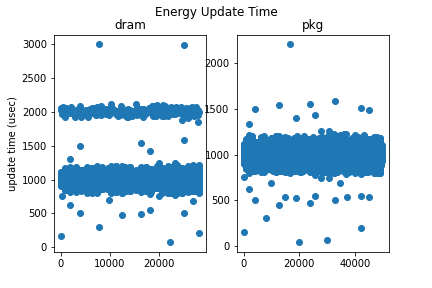
\includegraphics[width=10cm,height=10cm,keepaspectratio]{jmh/msr-update-rate/energy-update-time-simple.png}
    \caption{Energy Update Time (microseconds)}
    \label{fig:PKG-rapl-counter}
\end{figure}

% \begin{tabular}{lr}
\toprule
{} &          dram \\
\midrule
count &  28266.000000 \\
mean  &   1011.747860 \\
std   &    106.390894 \\
min   &     74.000000 \\
25\%   &    974.000000 \\
50\%   &   1000.000000 \\
75\%   &   1035.000000 \\
max   &   3070.000000 \\
\bottomrule
\end{tabular}

% \begin{tabular}{lr}
\toprule
{} &        dram.1 \\
\midrule
count &  49229.000000 \\
mean  &   1012.362896 \\
std   &    108.137976 \\
min   &     24.000000 \\
25\%   &    975.000000 \\
50\%   &   1000.000000 \\
75\%   &   1034.000000 \\
max   &   3031.000000 \\
\bottomrule
\end{tabular}

% \begin{tabular}{lr}
\toprule
{} &           pkg \\
\midrule
count &  49688.000000 \\
mean  &   1003.008694 \\
std   &     47.508242 \\
min   &     47.000000 \\
25\%   &    974.000000 \\
50\%   &   1000.000000 \\
75\%   &   1034.000000 \\
max   &   2198.000000 \\
\bottomrule
\end{tabular}

% \begin{tabular}{lr}
\toprule
{} &         pkg.1 \\
\midrule
count &  49689.000000 \\
mean  &   1002.989575 \\
std   &     47.588151 \\
min   &     24.000000 \\
25\%   &    974.000000 \\
50\%   &   1000.000000 \\
75\%   &   1033.000000 \\
max   &   1942.000000 \\
\bottomrule
\end{tabular}


These experiments confirm the expectation that the MSRs have a 1ms update rate, so all future sampling will happen at a 1ms rate, at minimum. 

Also worth noting that MSRs close off after several thousand repeated read attempts with no buffer time. \anote{What I meant by this: If you read the MSR over and over and over again with little to no other work in between, the MSR file shuts down and doesn't let you read any more. We had to put busywaits in our benchmarks to ``cool it off". This could be worth mentioning in that it solidifies the point that not only are you wasting time by sampling as fast as possible and trying for sub-millisecond periods, it also might temporarily ``break" the register to do it too often.}
\section{Results}

\subsection{Average Time Between Samples}
I did this for all benchmarks, but didn't parse and calculate individual averages per benchmarks. Just did average across benchmark, grouped by monitor type.
    \begin{figure}[H]
    	\centering
    	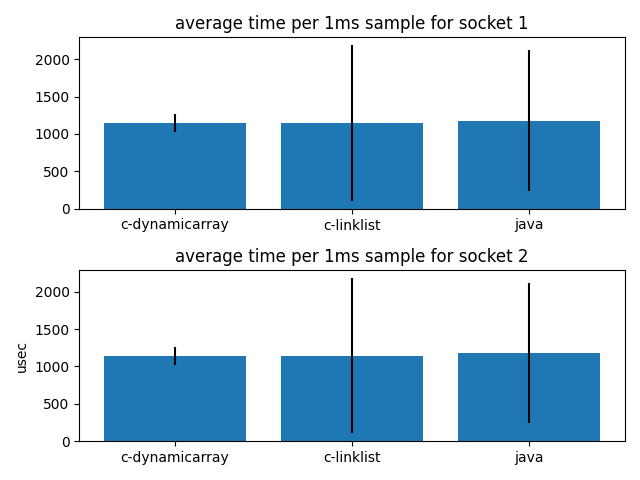
\includegraphics[width=17cm,height=17cm,keepaspectratio]{AsyncMonitorCompares/time-energy-persample/timestamp_average_usec_per-sample.png}
    	\caption{average reported usecs between 1 msec sample}
   	\label{fig:xalan-PKG-Time-scatter}
    \end{figure}

\subsection{Average Sample Energy}
I did this for all benchmarks, but didn't parse and calculate individual averages per benchmarks. Just did average across benchmark, grouped by monitor type.
    \begin{figure}[H]
    	\centering
    	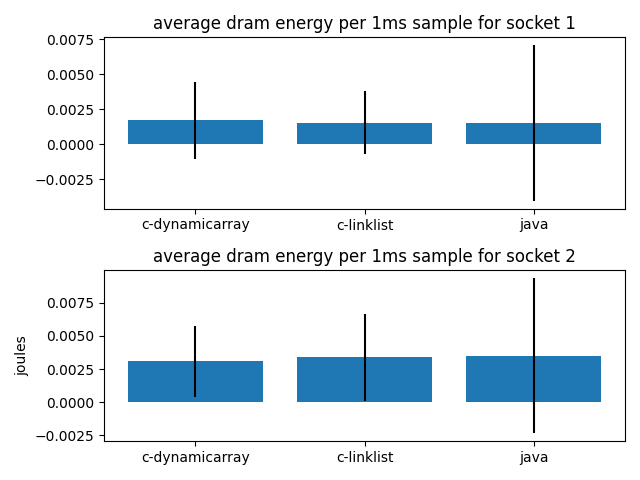
\includegraphics[width=17cm,height=17cm,keepaspectratio]{AsyncMonitorCompares/time-energy-persample/dram_average_joules_per-sample.png}
    	\caption{average energy per sample for dram}
   	\label{fig:xalan-PKG-Time-scatter}
    \end{figure}
    \begin{figure}[H]
    	\centering
    	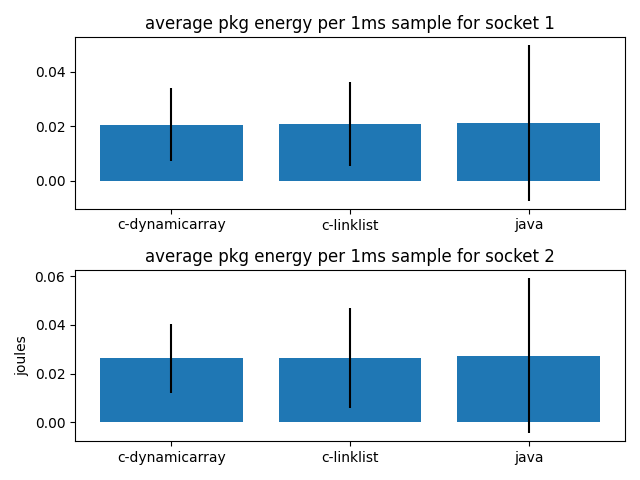
\includegraphics[width=17cm,height=17cm,keepaspectratio]{AsyncMonitorCompares/time-energy-persample/pkg_average_joules_per-sample.png}
    	\caption{average energy per sample for pkg}
   	\label{fig:xalan-PKG-Time-scatter}
    \end{figure}
    
\subsection{JNI Runtime Overhead}
    The graphs below are histograms. X axis is the microsecond runtimes, Y axis is how many readings we got
    for that runtime. Crazy high values (more than 3 standard deviations from the mean) are removed because they are relatively few and that stretch the graph and make it illegible. But we still captured
    them in the Python script, because they're probably important information and intend to render them somehow.

    It appears that creating a \texttt{jstring} and rendering it in Java as a \texttt{String} is has notable time overhead and variance as well.
    
    It seems that while a JNI call itself does not incur overhead, as demonstrated with similar runtimes for our void-returning native methods, our method that returns a string of energy data has a considerable runtime increase from simply calling the C side function. So creation of a Java string in C, and then passing it to Java, provides a notable cost, both in time of execution and in variance of the time. \todo{finalize the results from that recent test you did, see how it goes in terms of substantiating this}
    
    \anote{Should I also note that on my 1-socket computer the JNI overhead is a lot lower? It's probably because I'm returning less data, so the object I build is smaller.}
    
    \begin{figure}[H]
	    \centering
	    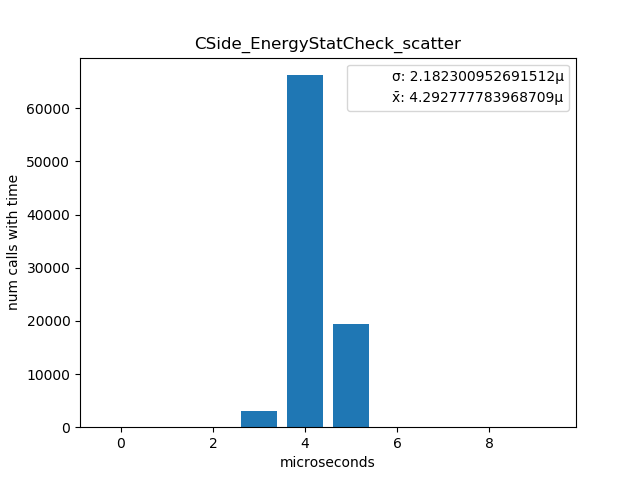
\includegraphics[width=10cm,height=10cm,keepaspectratio]{jmh/jni-overhead/CSide_EnergyStatCheck_scatter.png}
	    \caption{Runtime for EnergyStatCheck on CSide}
	    \label{fig:jolteon-jmh-runtime-energystatcheck-c}
    \end{figure}
    \begin{figure}[H]
	    \centering
	    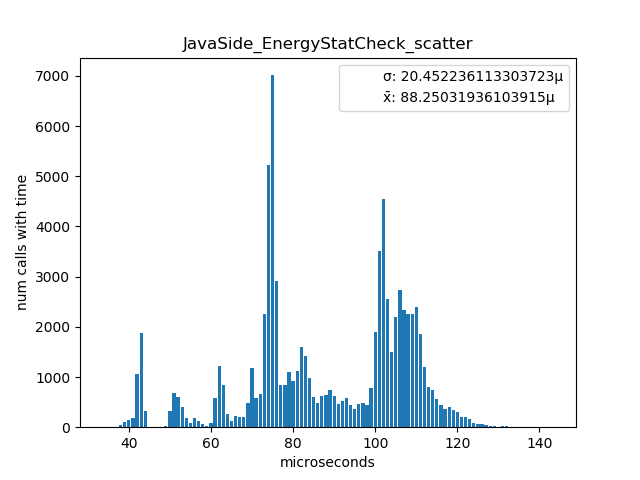
\includegraphics[width=10cm,height=10cm,keepaspectratio]{jmh/jni-overhead/JavaSide_EnergyStatCheck_scatter.png}
	    \caption{Runtime for EnergyStatCheck on JavaSide}
	    \label{fig:jolteon-jmh-runtime-energystatcheck-java}
    \end{figure}
    
    \begin{figure}[H]
	    \centering
	    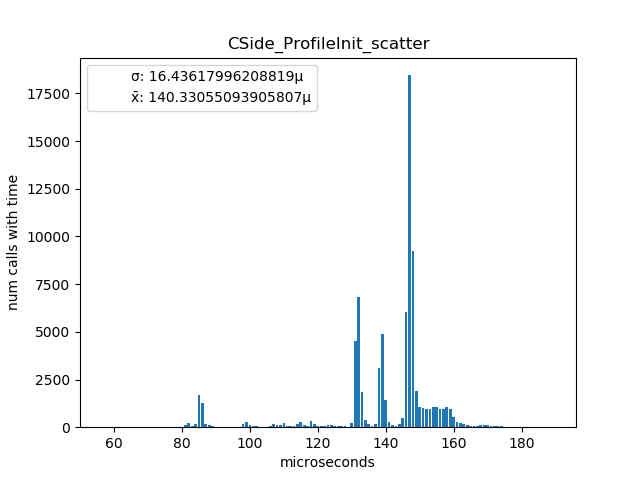
\includegraphics[width=10cm,height=10cm,keepaspectratio]{jmh/jni-overhead/CSide_ProfileInit_scatter.png}
	    \caption{Runtime for ProfileInit on CSide}
	    \label{fig:jolteon-jmh-runtime-profileinit-c}
    \end{figure}
    \begin{figure}[H]
	    \centering
	    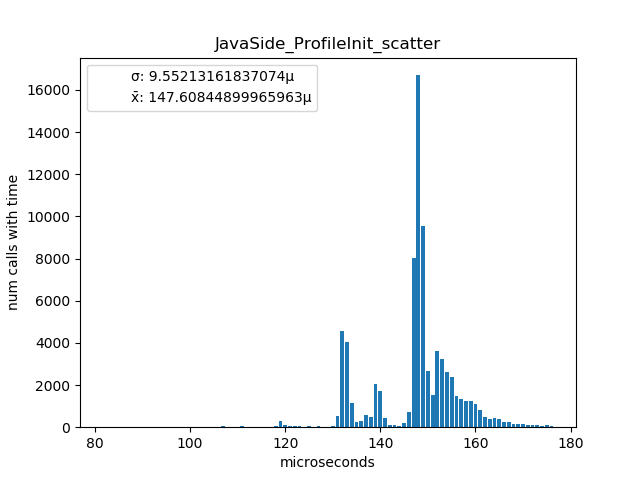
\includegraphics[width=10cm,height=10cm,keepaspectratio]{jmh/jni-overhead/JavaSide_ProfileInit_scatter.png}
	    \caption{Runtime for ProfileInit on JavaSide}
	    \label{fig:jolteon-jmh-runtime-profileinit-java}
    \end{figure}

    \begin{figure}[H]
	    \centering
	    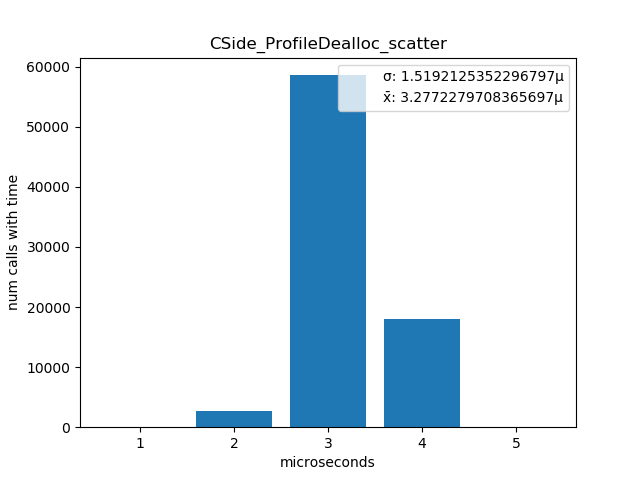
\includegraphics[width=10cm,height=10cm,keepaspectratio]{jmh/jni-overhead/CSide_ProfileDealloc_scatter.png}
	    \caption{Runtime for ProfileDealloc on CSide}
	    \label{fig:jolteon-jmh-runtime-profileDealloc-c}
    \end{figure}
    \begin{figure}[H]
	    \centering
	    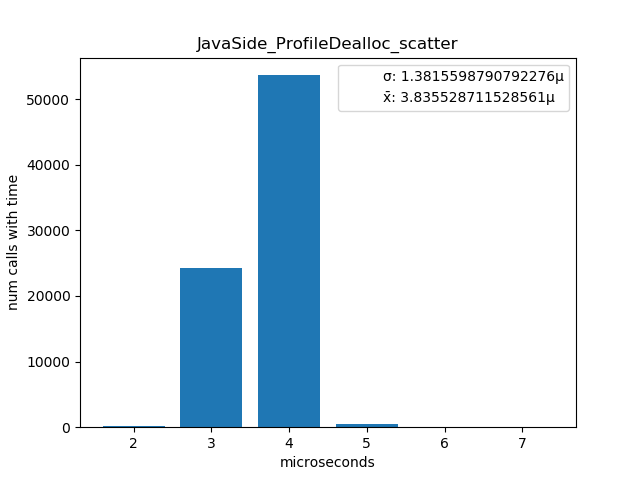
\includegraphics[width=10cm,height=10cm,keepaspectratio]{jmh/jni-overhead/JavaSide_ProfileDealloc_scatter.png}
	    \caption{Runtime for ProfileDealloc on JavaSide}
	    \label{fig:jolteon-jmh-runtime-profileDealloc-java}
    \end{figure}

\subsection{Time to Read One Energy Value from MSR}
    It's all hovering around one microsecond, with occasional relatively-high values. Values greater than 3 standard deviations weren't plotted because it makes the graph illegible, but we still captured them
    in the Python script and intend to represent them somehow, because it's still probably good to know
    that we'll very occasionally get super high runtimes.
    
    Graphs below are histograms. X axis is the runtime, Y axis is how many readings we found at that runtime.
    
    \begin{figure}[H]
	    \centering
	    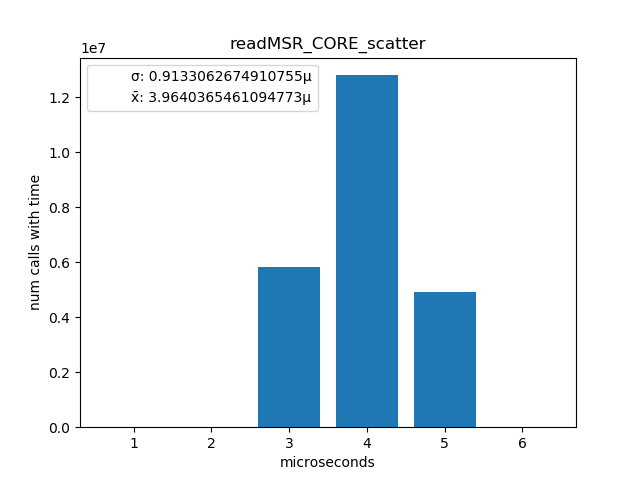
\includegraphics[width=10cm,height=10cm,keepaspectratio]{jmh/readmsr-runtime/readMSR_CORE_scatter.png}
	    \caption{Runtime to read MSR for CORE RAPL counter}
	    \label{fig:CORE-rapl-counter}
    \end{figure}
    
    \begin{figure}[H]
	    \centering
	    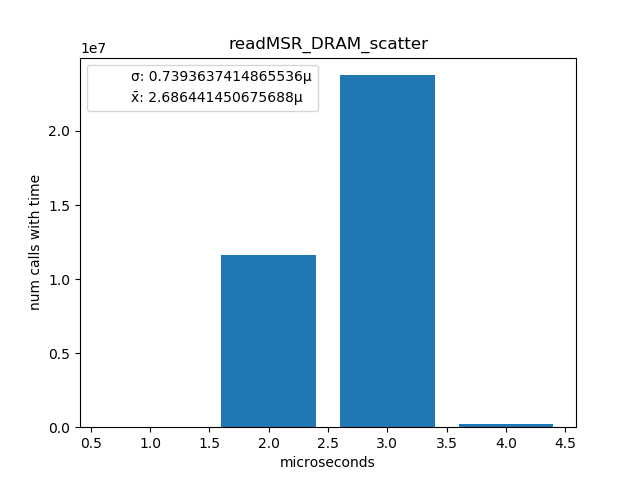
\includegraphics[width=10cm,height=10cm,keepaspectratio]{jmh/readmsr-runtime/readMSR_DRAM_scatter.png}
	    \caption{Runtime to read MSR for DRAM RAPL counter}
	    \label{fig:DRAM-rapl-counter}
    \end{figure}
    
    \begin{figure}[H]
	    \centering
	    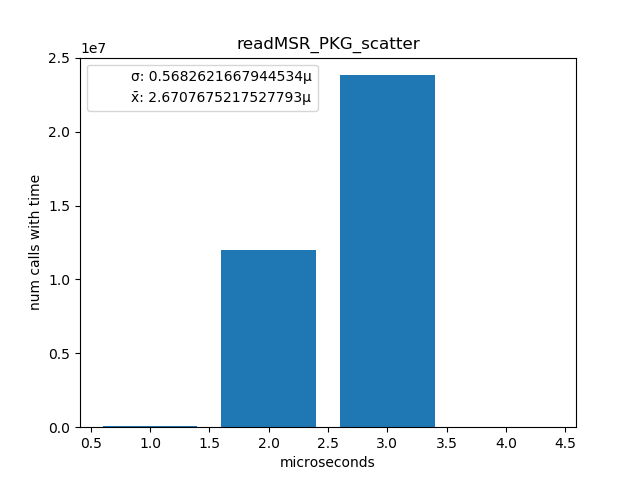
\includegraphics[width=10cm,height=10cm,keepaspectratio]{jmh/readmsr-runtime/readMSR_PKG_scatter.png}
	    \caption{Runtime to read MSR for PKG RAPL counter}
	    \label{fig:PKG-rapl-counter}
    \end{figure}
    
    %\begin{figure}[H]
	%    \centering
	%    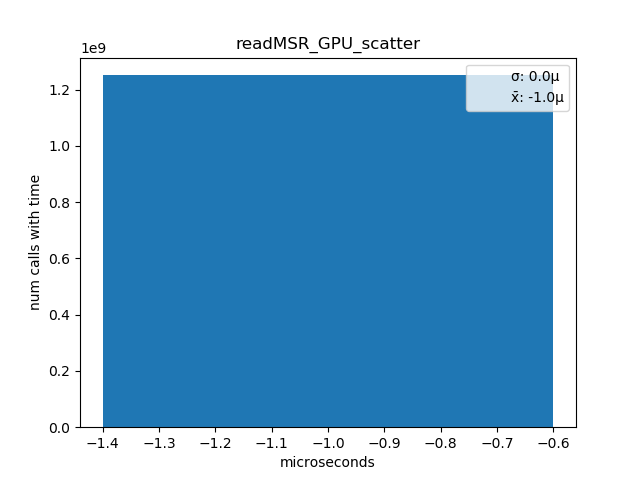
\includegraphics[width=10cm,height=10cm,keepaspectratio]{jmh/readmsr-runtime/readMSR_GPU_scatter.png}
	%    \caption{Runtime to read MSR for GPU RAPL counter}
	%    \label{fig:GPU-rapl-counter}
    %\end{figure}
    

\subsection{Java SyncEnergyMonitor Sampling Runtime}
This part is to show the runtime of taking a whole sample. This can serve to show the time overhead of simply taking a sample, the whole difference between Java and C for sampling (other experiments just isolate the JNI portion of the overhead), and the runtime of the three different types of samples that are taken: raw string sample, primitive array sample, and object sample.

Object sample vs primitive sample runtime is useful for people to know if they're thinking about the tradeoff. There's pretty clearly going to be a memory difference (obviously), but also runtime could be useful. (Make sure you confirm the difference in runtime that you just observed).

String sample is (maybe) relevant because Java Side Async Monitor directly stores the string samples, so we can compare this sampling runtime with the C side runtime. Can make for explanations about performance difference between C and Java side Async Monitors. However, this method is package private and we covered a close-enough situation in the JNI runtime overhead, so it might be better to just look at that.

JMH experiment: 7 warmups, 30 iterations, 10 second period for warmup and iteration. As many shots as possible per iteration (with 100-count busywait, so MSRs dont shut down), takes the average of the runtime in microseonds.

    \begin{figure}[H]
	    \centering
	    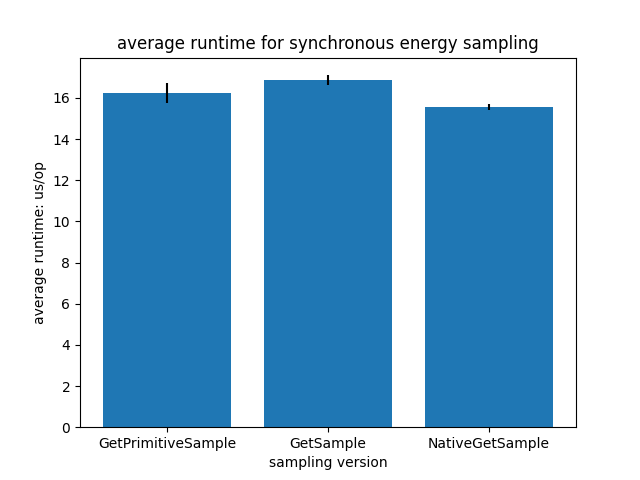
\includegraphics[width=10cm,height=10cm,keepaspectratio]{jmh/syncmonitor/sync-samples-runtime.png}
	    \caption{Runtimes per sampling function}
	    \label{fig:PKG-rapl-counter}
    \end{figure}

While there is a predictable difference in overhead run time, it is all within the range of a single microsecond. Memory could be a consideration for whether or not a primitive array or object wrapper should be used to represent an energy sample, but in most cases, runtime should not.

\subsection{AsyncEnergyMonitor Comparison}
\subsubsection{Sampling Efficiency}
Comparing how efficient the sampling is for each monitor. Divide number of samples collected
by msec lifetime of monitor. The first graph is average for the 20 benchmark iterations and
the second is average per monitor across all iterations.

    \begin{figure}[H]
    	\centering
    	\includegraphics[width=17cm,height=17cm,keepaspectratio]{AsyncMonitorCompares/sampling-efficiency_perbench.png}
    	\caption{Average sampling efficiency per benchmark}
    	\label{fig:samplingefficiency_perbench}
    \end{figure}
    \begin{figure}[H]
    	\centering
    	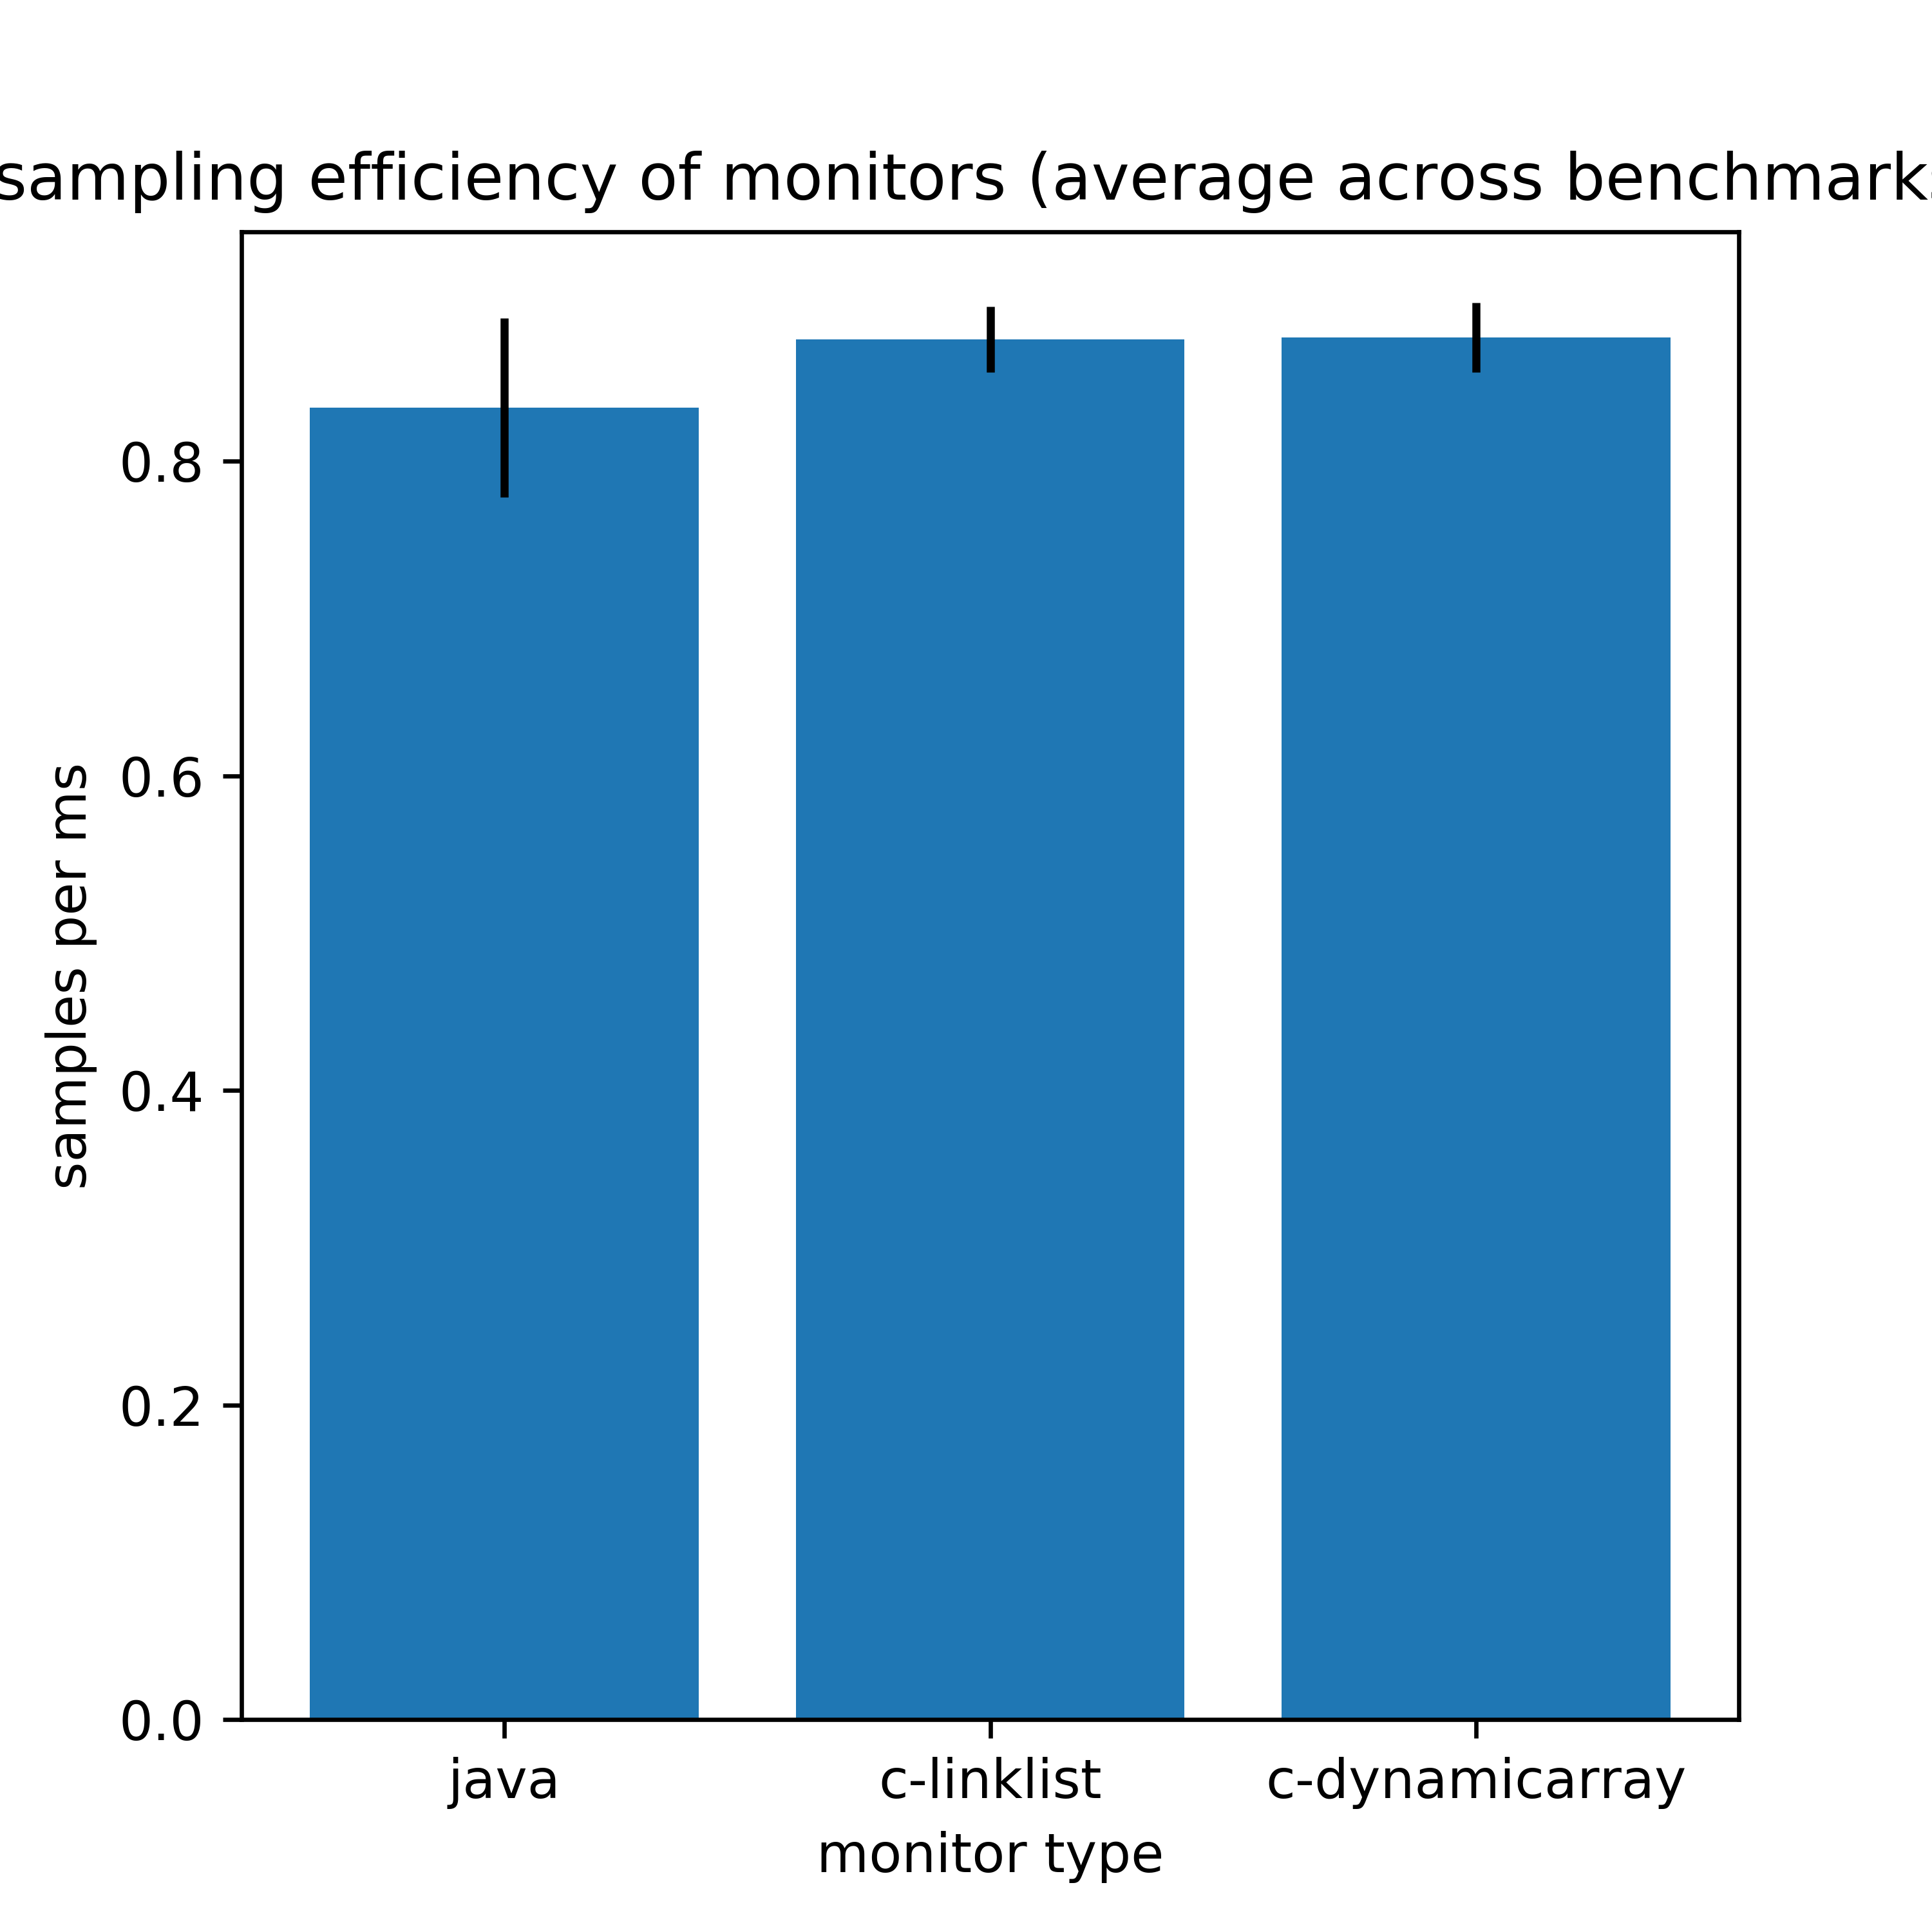
\includegraphics[width=17cm,height=17cm,keepaspectratio]{AsyncMonitorCompares/sampling-efficiency_overall.png}
    	\caption{Average sampling effieicency across all benchmarks}
    	\label{fig:samplingefficiency_overall}
    \end{figure}

Looks like Java is (slightly) less efficient, since sampling takes longer, as evidenced by
our JNI runtime overhead experiment. The wider error bar on the Java monitor makes sense. Looks
like it's a bit less precise in its sampling rate then.

\begin{verbatim} 
Raw Numbers
overall_java_avg: 0.8339
overall_java_std: 0.0569

overall_c_ll_avg: 0.8775
overall_c_ll_std: 0.0210

overall_c_da_avg: 0.8786
overall_c_da_std: 0.0222
\end{verbatim} % in case the actual numbers are useful at all

In conclusion, the C monitors are comparable in sampling efficiency, and both a bit better than
the Java one.

\subsection{Memory Footprint}
\anote{These results are definitely not accurate. I figured out some issues in my calculations, and the results are different. However, I can't upload the complete results because Jolteon is down. I have 3 iterations saved on my machine as standin data while I write my scripts, but data for all 25 iterations is currently unreachable until Jolteon gets fixed, so I can't run the analysis there and get new results.}

Below graph is the percent difference of memory added by having the AsyncEnergyMonitor active vs no monitor active. This is an average across all benchmarks.

    \begin{figure}[H]
    	\centering
    	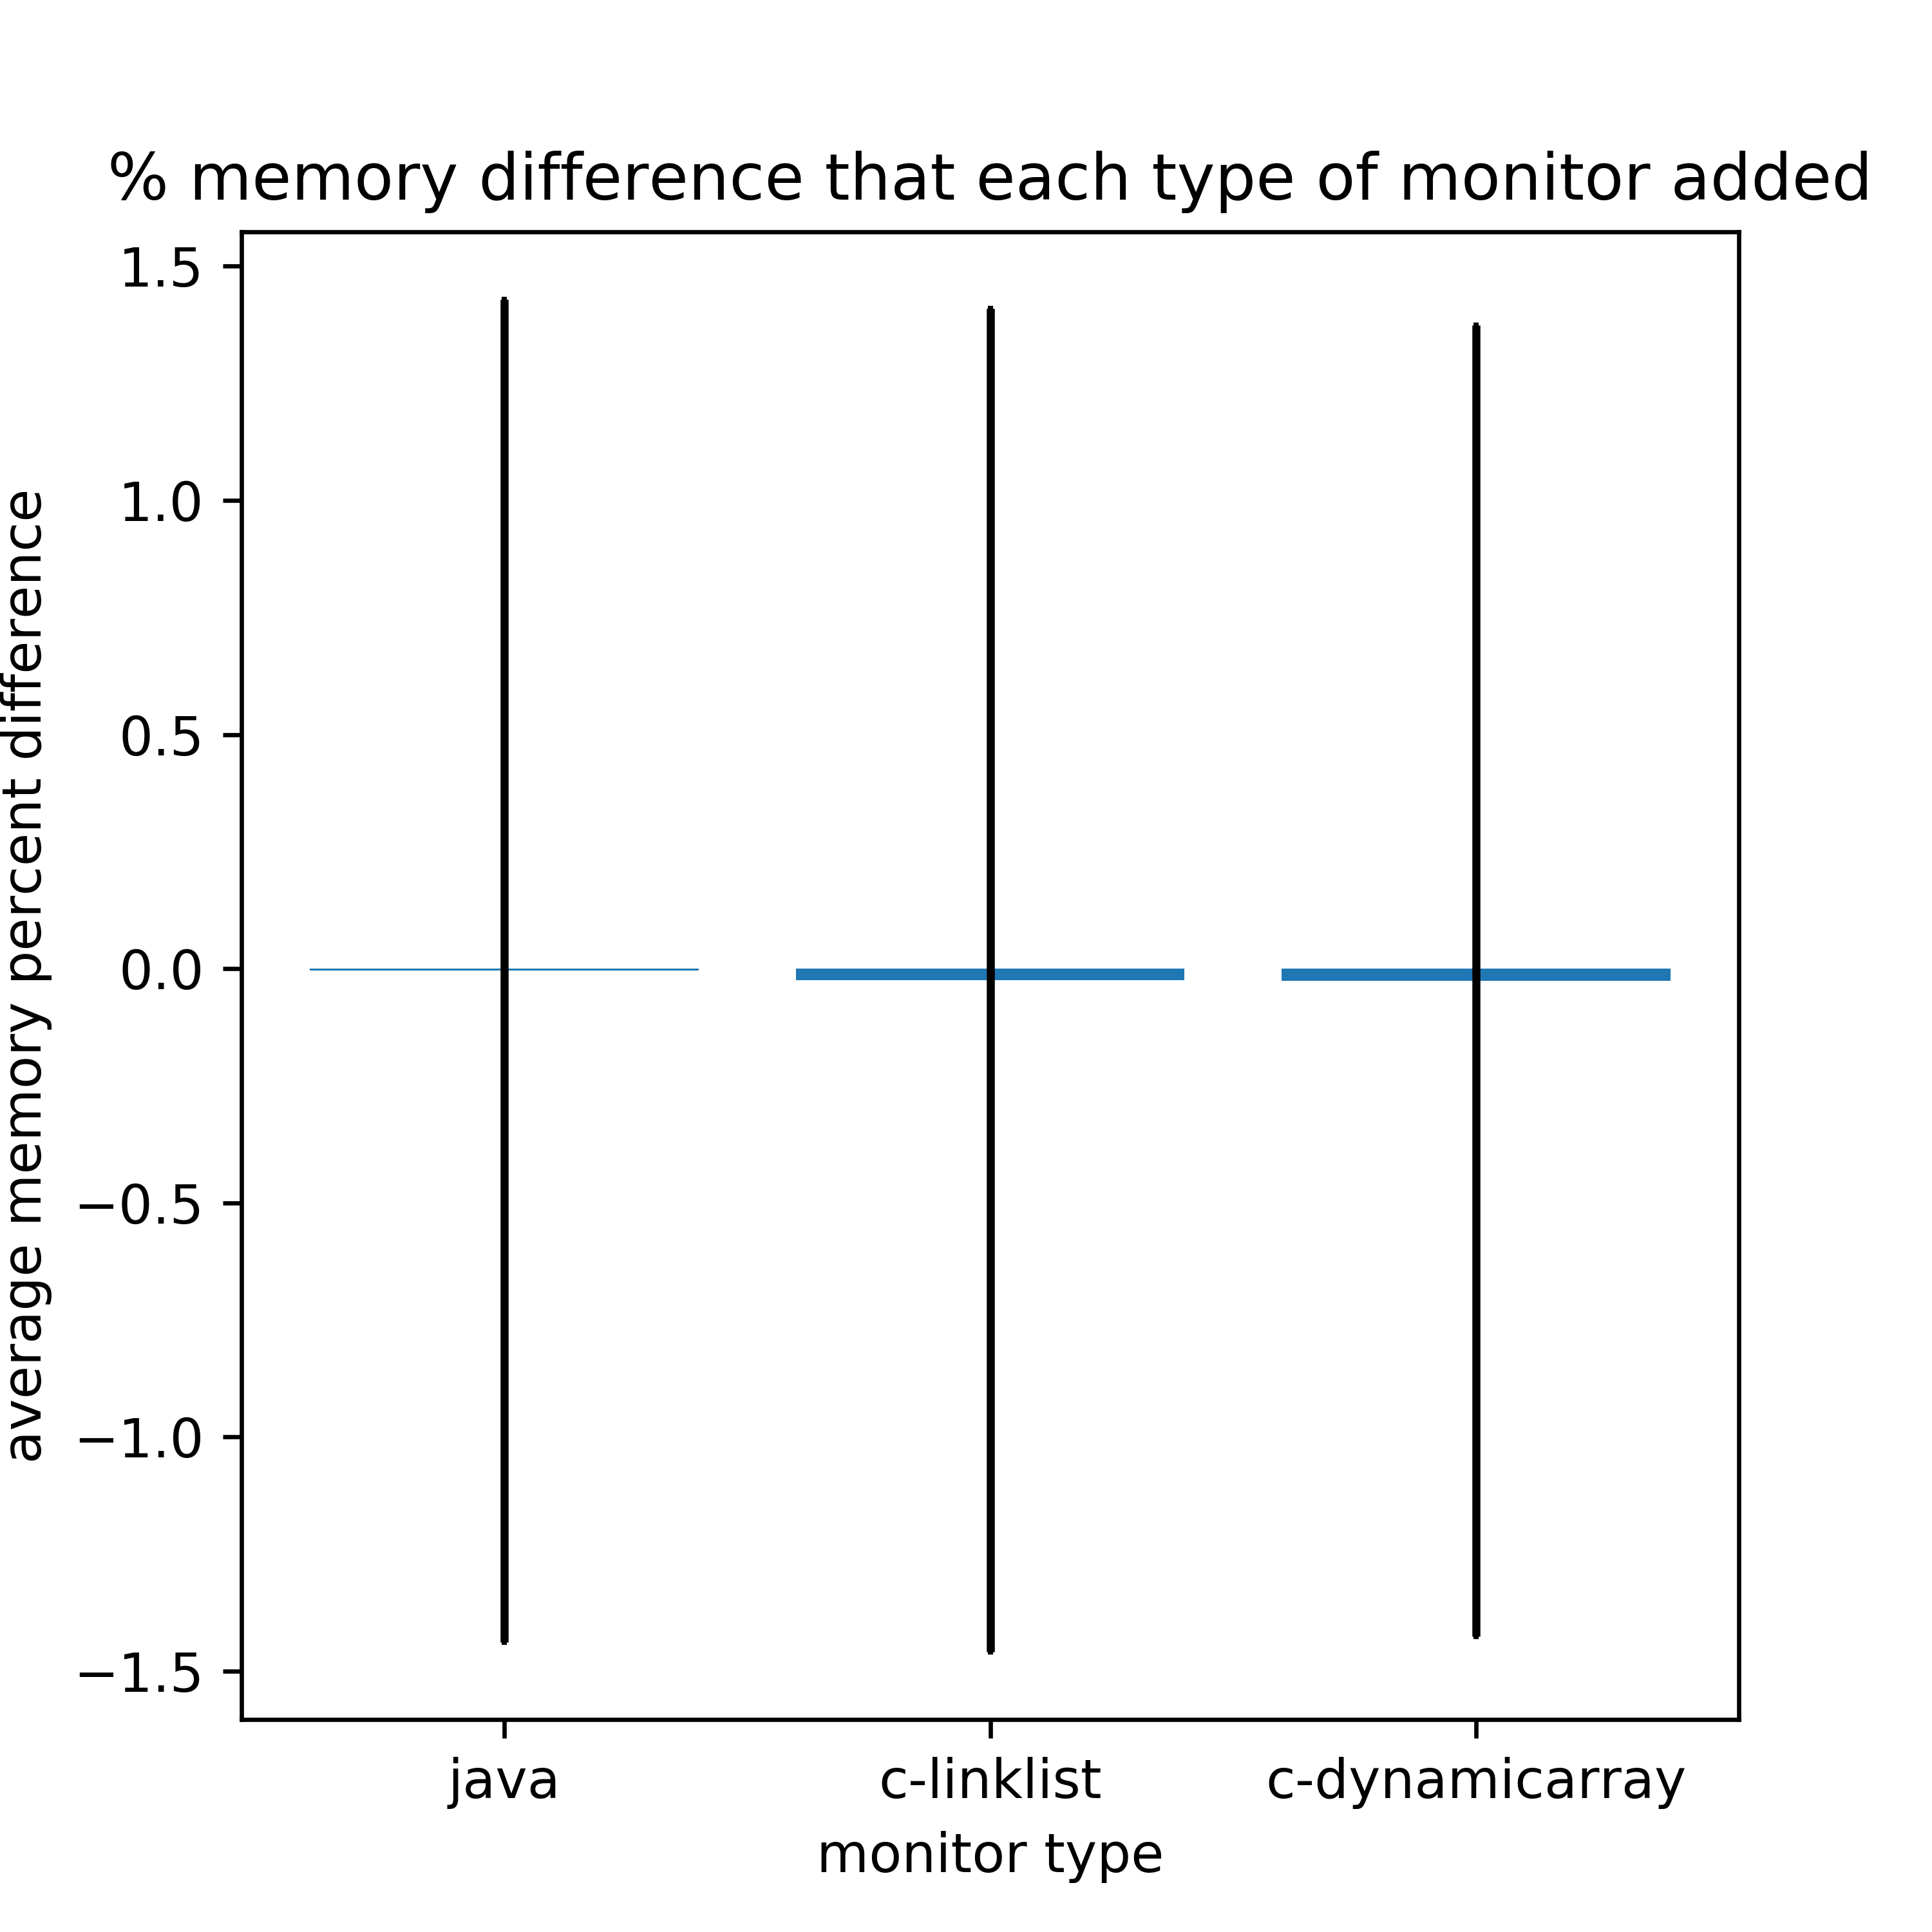
\includegraphics[width=17cm,height=17cm,keepaspectratio]{AsyncMonitorCompares/memory-compare_overall.png}
    	\caption{Memory Overhead of Each Monitor Type}
    	\label{fig:samplingefficiency_perbench}
    \end{figure}

The difference between the monitors (and the overall memory footprint) is extraordinarily negligible. This makes sense, since an energy monitor is effectively just a list of numbers in memory, it's just more fancy seeming because it gets updated asynchronously. But it's just energy readings and timestamps, so it's small potatoes in the grand scheme of things.

\anote{So the C monitors do tend have a slightly lower footprint, since a C sample stored in the monitor is a struct, while the Java sample is the string returned from native memory (if we parsed it into a primitive sample, it would have lower memory footprint but each sample would take even longer to generate). But as this experiment shows, it's all small potatoes compared to the total memory consumption of the benchmarks. So, is the smaller C memory worth writing about? Are there super memory sensitive Java situations that this is notable for?}

\anote{Should I talk about and try to explain the negative percent differences? Both the C monitors are slightly below 0...}

\section{Proposed other experiments}
    I wanted to suggest these as possible experiments / software improvements. Let me know what you think.

    \subsection{Better C side sleeping}
        \textbf{Not precise to microseconds.} Precise at ms, but, sleeping for 1ms doesn't actually take 1000us. Around 1100 or so on average. This is bad if repeatedly taking samples, as the extra time adds up and you get less samples than you expect, if you're sleeping for single digit ms times. You'd expect 1000 samples per second if sleeping at 1ms, but you don't get that many.
        
        There are more precise timers in C that I could try to implement, Timur showed me a thing that I could see if it works here.
        
    \subsection{Shrinking the size of the data brought across the JNI}
        I've noticed that the size of the string I bring across the JNI has a significant impact on JNI overhead; on Jolteon, samples take longer because I'm returning data for 2 sockets, so the string is longer.
        
        I could experiment with serializing the data in a binary format instead of a human readable format, and then parsing it on the Java side. Something like a byte array, or a string where each character is a byte of the C-side energy sample struct. That should make the data passed from C to java a lot smaller, reducing JNI overhead.
        
        This might be more work than it's worth though. Can revisit once all of the runtime results are put up. I'll put up runtime on my single socket computer, and runtime on the double socket computer (also, do we ever expect servers with mutiple sockets? because if we have 4 or 8 sockets, the readings are going to be even bigger, which could be even more runtime!
        
        If we need a specific demonstration of how long it takes to bring different string sizes across the JNI, i can set up a JMH experiment for that, although that might be overkill.

\section{Appendix}

\anote{Right now this is just a dump of stuff that I may or may not include in the appendix, will fix it up as things develop.}

\subsection{Memory Footprint of Object Sample vs Primitive Array Sample}
\anote{So it's my understanding that comparing the memory footprint of these two representations
of the energy samples is not useful, since the specific numbers vary based on the own user's
runtime, and users will already know that they're doing a convenience vs memory tradeoff. Just
want to confirm that these results aren't useful before I delete this.}

Used the classmexer agent provided at https://javamex.com/classmexer/

It uses instrumentation to get the memory usage of an object, so the object header
(12 bytes) and the size of all of its fields. I made sure to ask for deep memory
usage, so if its fields are non-primitive types, we also get the number of bytes
in the entire object, not just of the reference stored in the top level object. Java
object sizes are padded up to the next multiple of 8. Units are bytes.

Below is the output of my test program, where I took an array sample and an object
sample, and got the deep memory use of each.
\begin{verbatim}

For raw stamp sample:
  primitive sample: 48 bytes
  object sample: 96 bytes
    [1164.4618, 184.5864, 4048.8065, 11751.1702]
    1164.4625,184.5864,4048.8231,11751.1893,1619625664691708

For diff sample (over a 100ms delay):
  primitive sample: 48 bytes
  object sample: 96 bytes
    [0.017399999999952342, 0.0, 0.16520000000036816, 0.30240000000048894]
    0.0235,0.0096,0.0237,0.1486,101030
    
\end{verbatim}

These results are on my computer, since Jolteon currently has my other experiments
running, so we'd get other values since it's a 2socket/3power-domain machine, as opposed to my 1socket/4power-domain machine.

Math checks out. Primitive sample is header (12 bytes) + 4 doubles (32 bytes) =
44, rounded up to 48.
Object sample is header (12) + primitive sample (44 +4padding) + Instant(12 + 8 + 8) = 88, round up to 96.

\textbf{66\% percent difference} in sizes of these implementations

\subsection{MSR update rate extra plots}
%\subsubsection{MSR Updates Extra}

%Here we continue exploring the data collected from MSR update experiment based on
%Timur's suggestions.

%Timur also suggested we create autocorrelation plots, for which I have written code, but I am not sure how to read them or whether I am creating them correctly, so I have not added them to the document. %% Rutvik did this, I can ask him about it in a few days when he's done taking part in
%% all of the shenanigans of his cousin's wedding

There is also a summary of the statistics relating to correlation between different values which I was not able to add to the document because of formatting errors. %% Also Rutvik, will ask him
%% where to find the data, once he's freed up.

\begin{figure}[H]
    \centering
    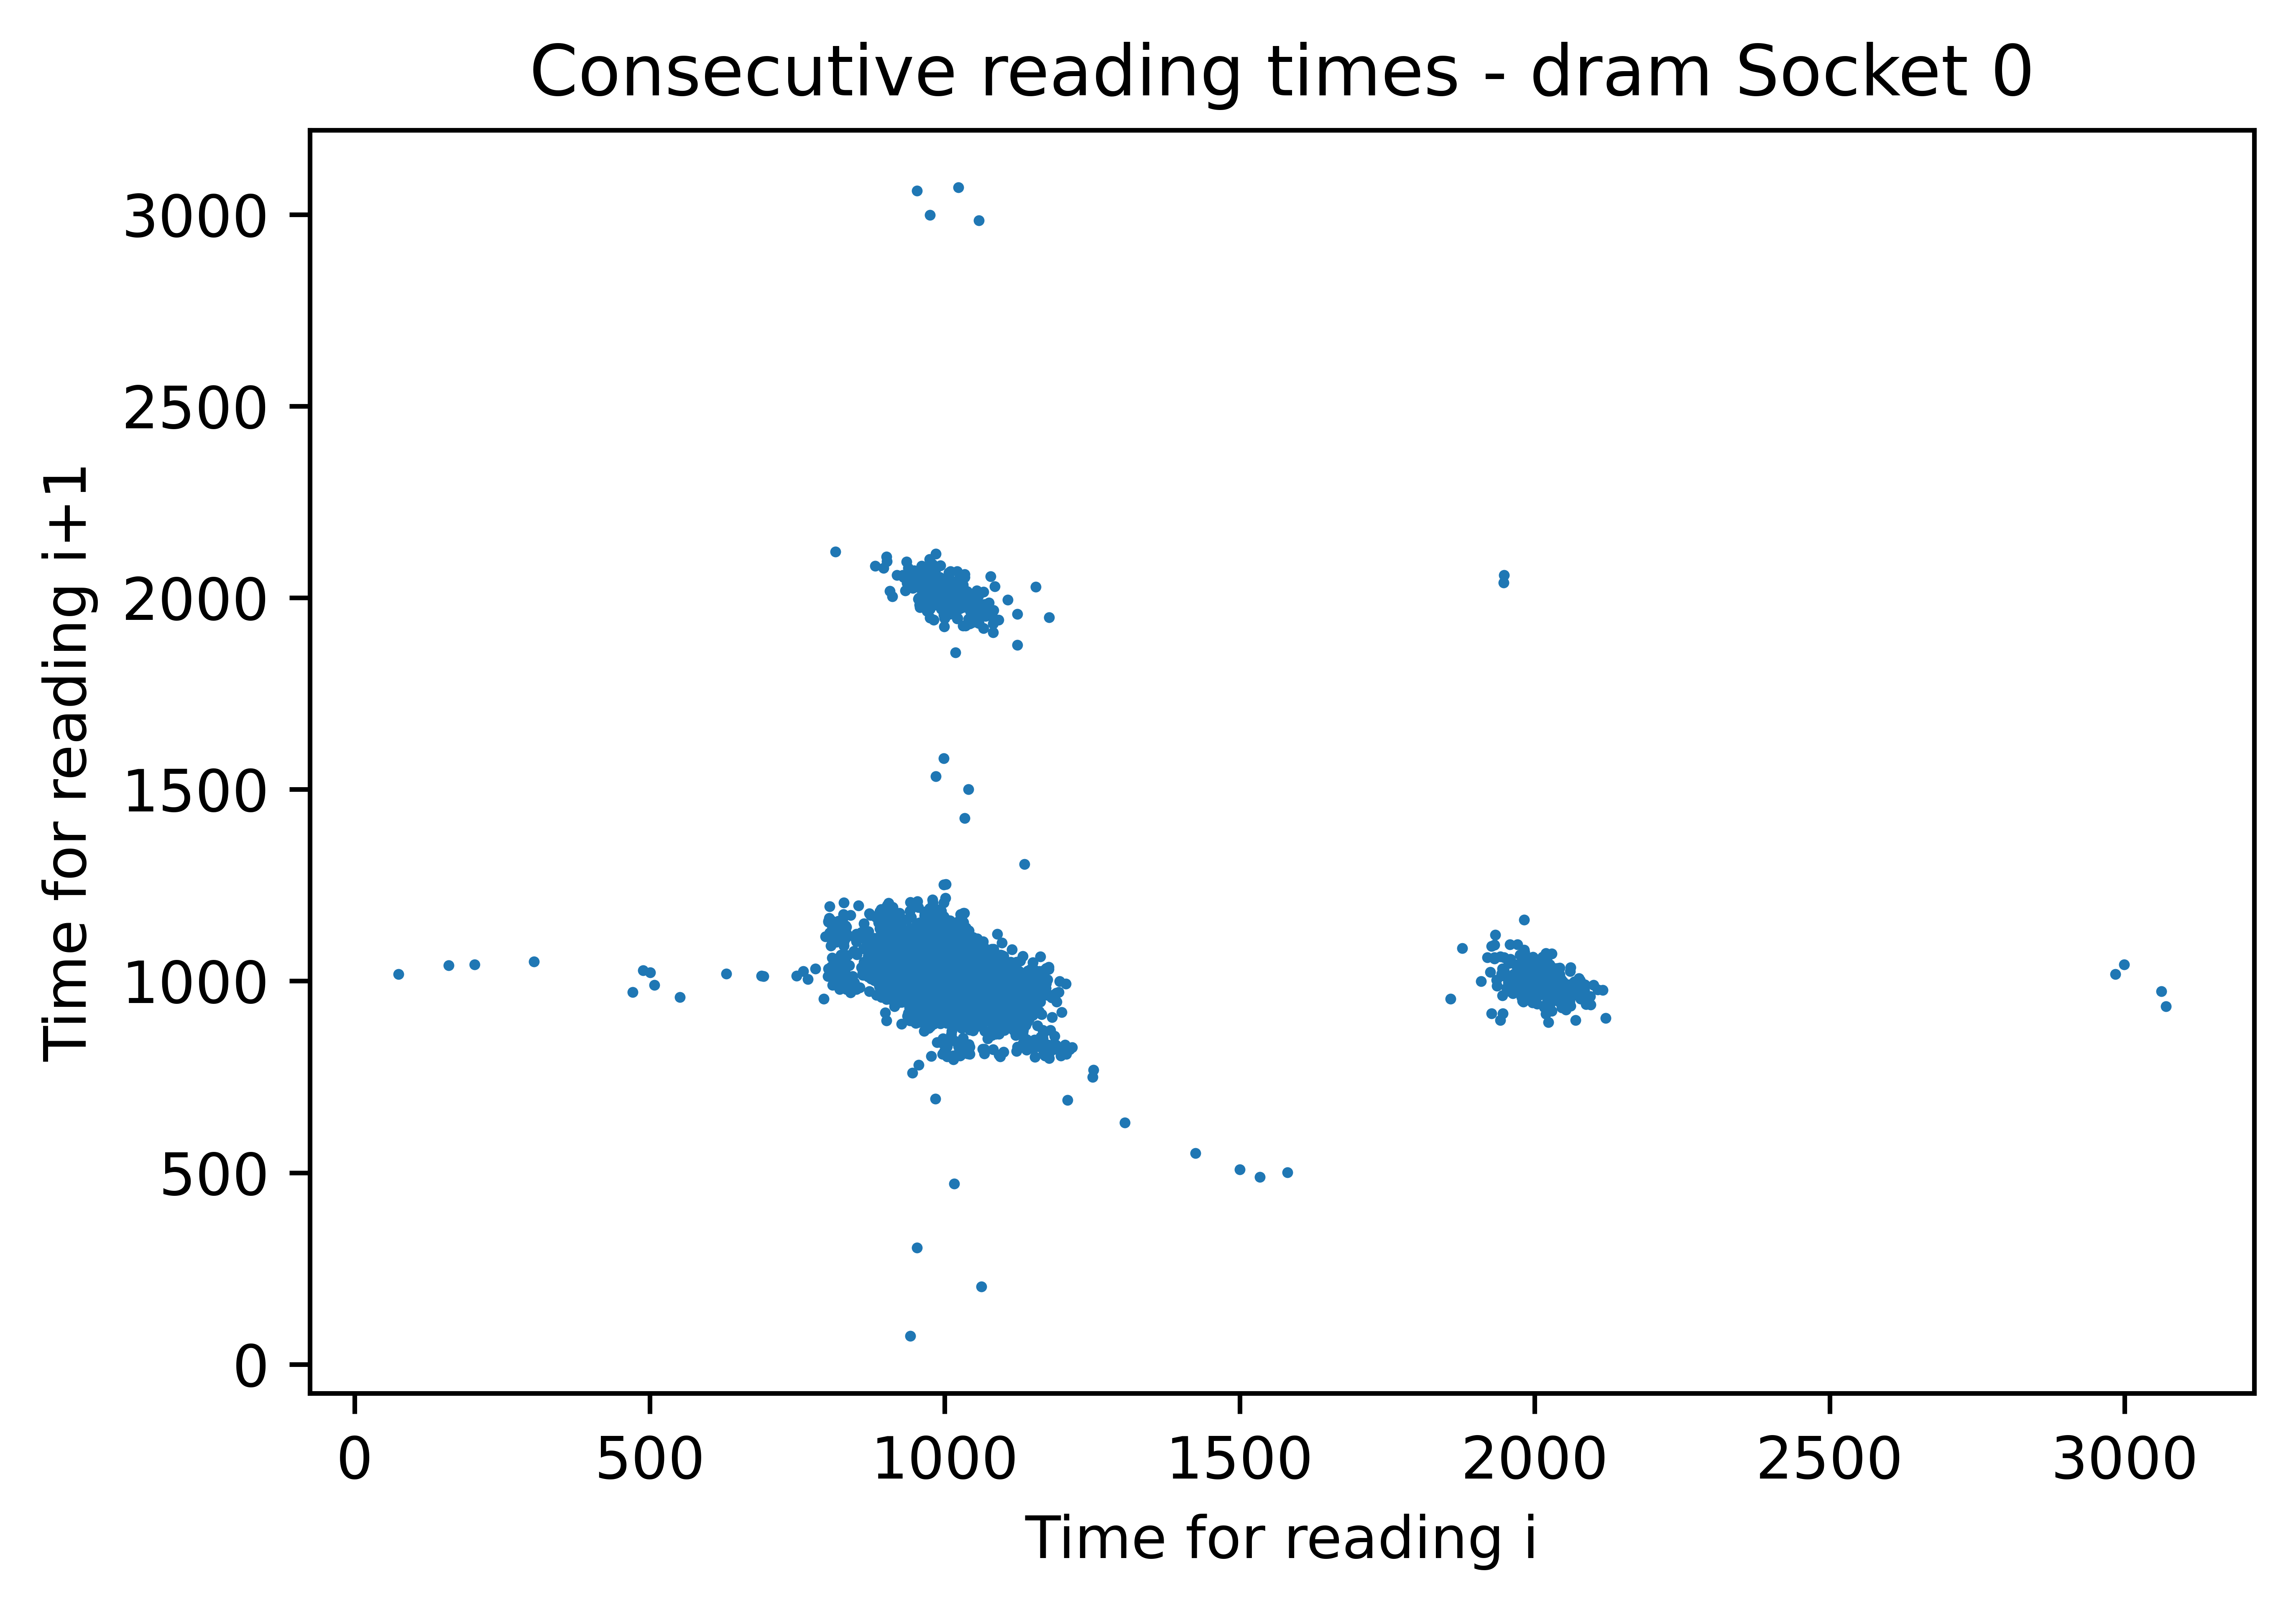
\includegraphics[width=10cm,height=10cm,keepaspectratio]{jmh/msr-update-rate/dram_Socket_0-i_n-v-i_n1.png}
    \caption{How long it takes for the PKG\_socket2 MSR to update (microseconds)}
    \label{fig:PKG-rapl-counter}
\end{figure}

\begin{figure}[H]
    \centering
    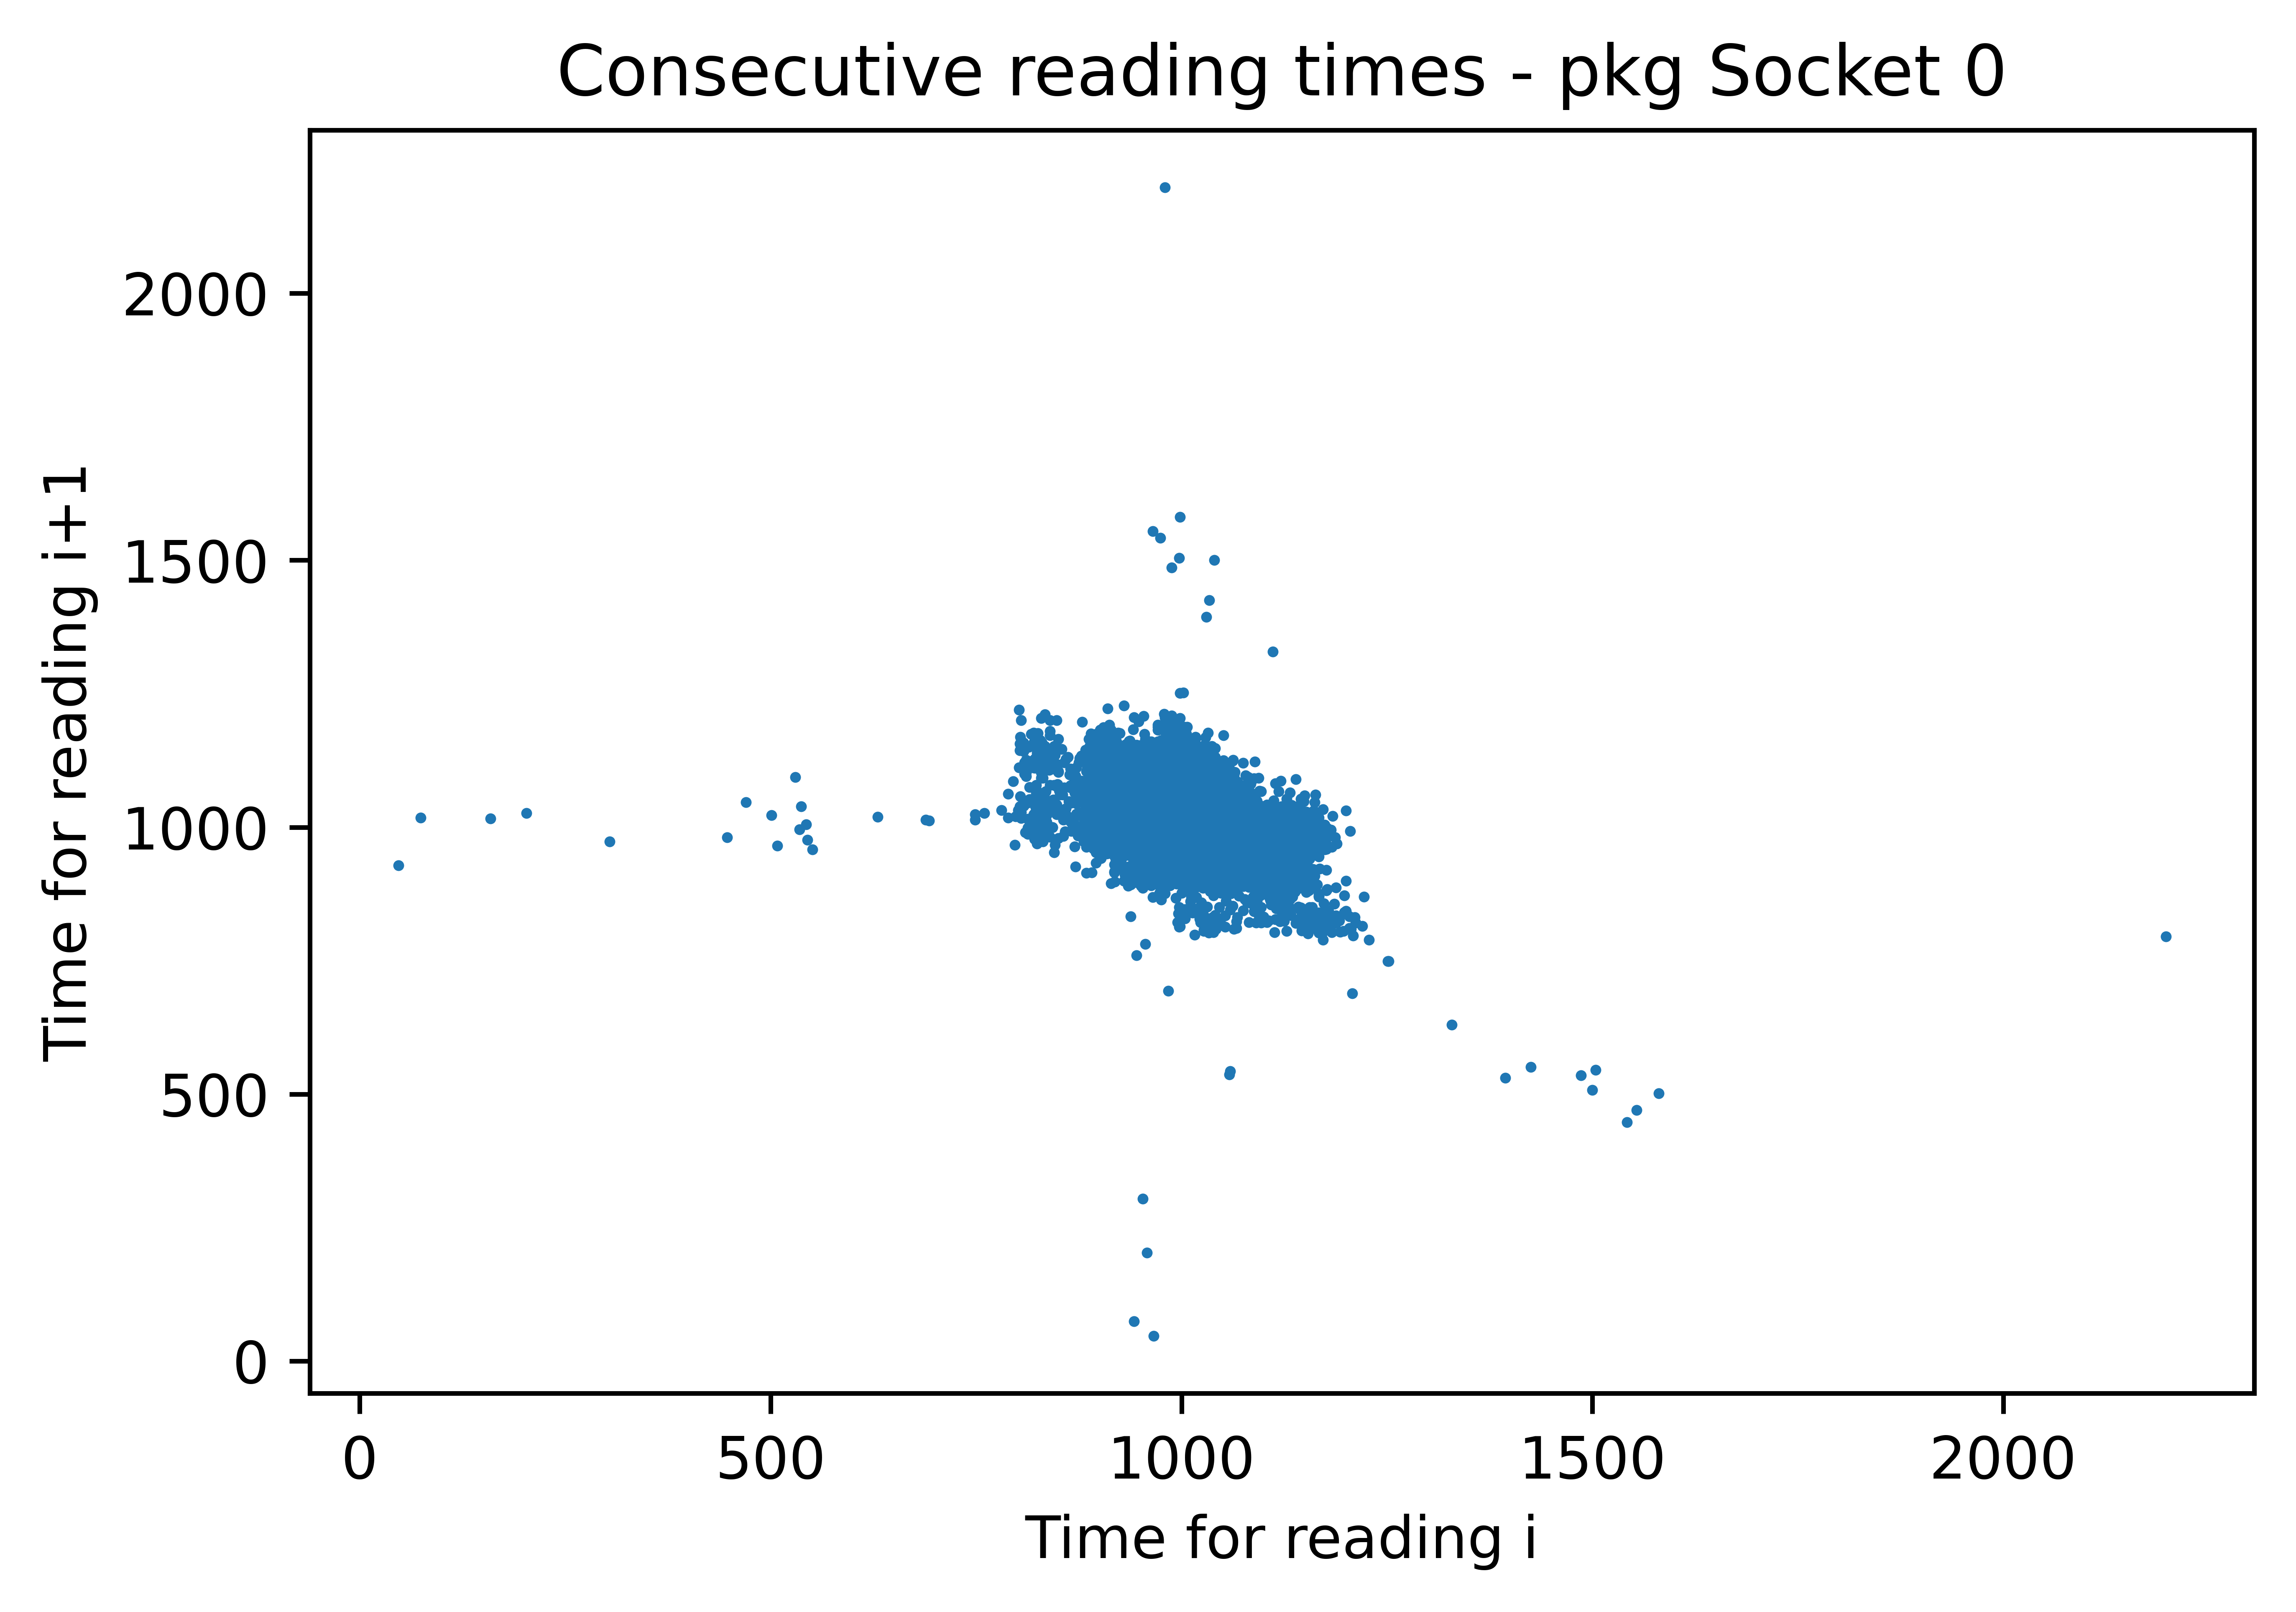
\includegraphics[width=10cm,height=10cm,keepaspectratio]{jmh/msr-update-rate/pkg_Socket_0-i_n-v-i_n1.png}
    \caption{How long it takes for the PKG\_socket2 MSR to update (microseconds)}
    \label{fig:PKG-rapl-counter}
\end{figure}

\begin{figure}[H]
    \centering
    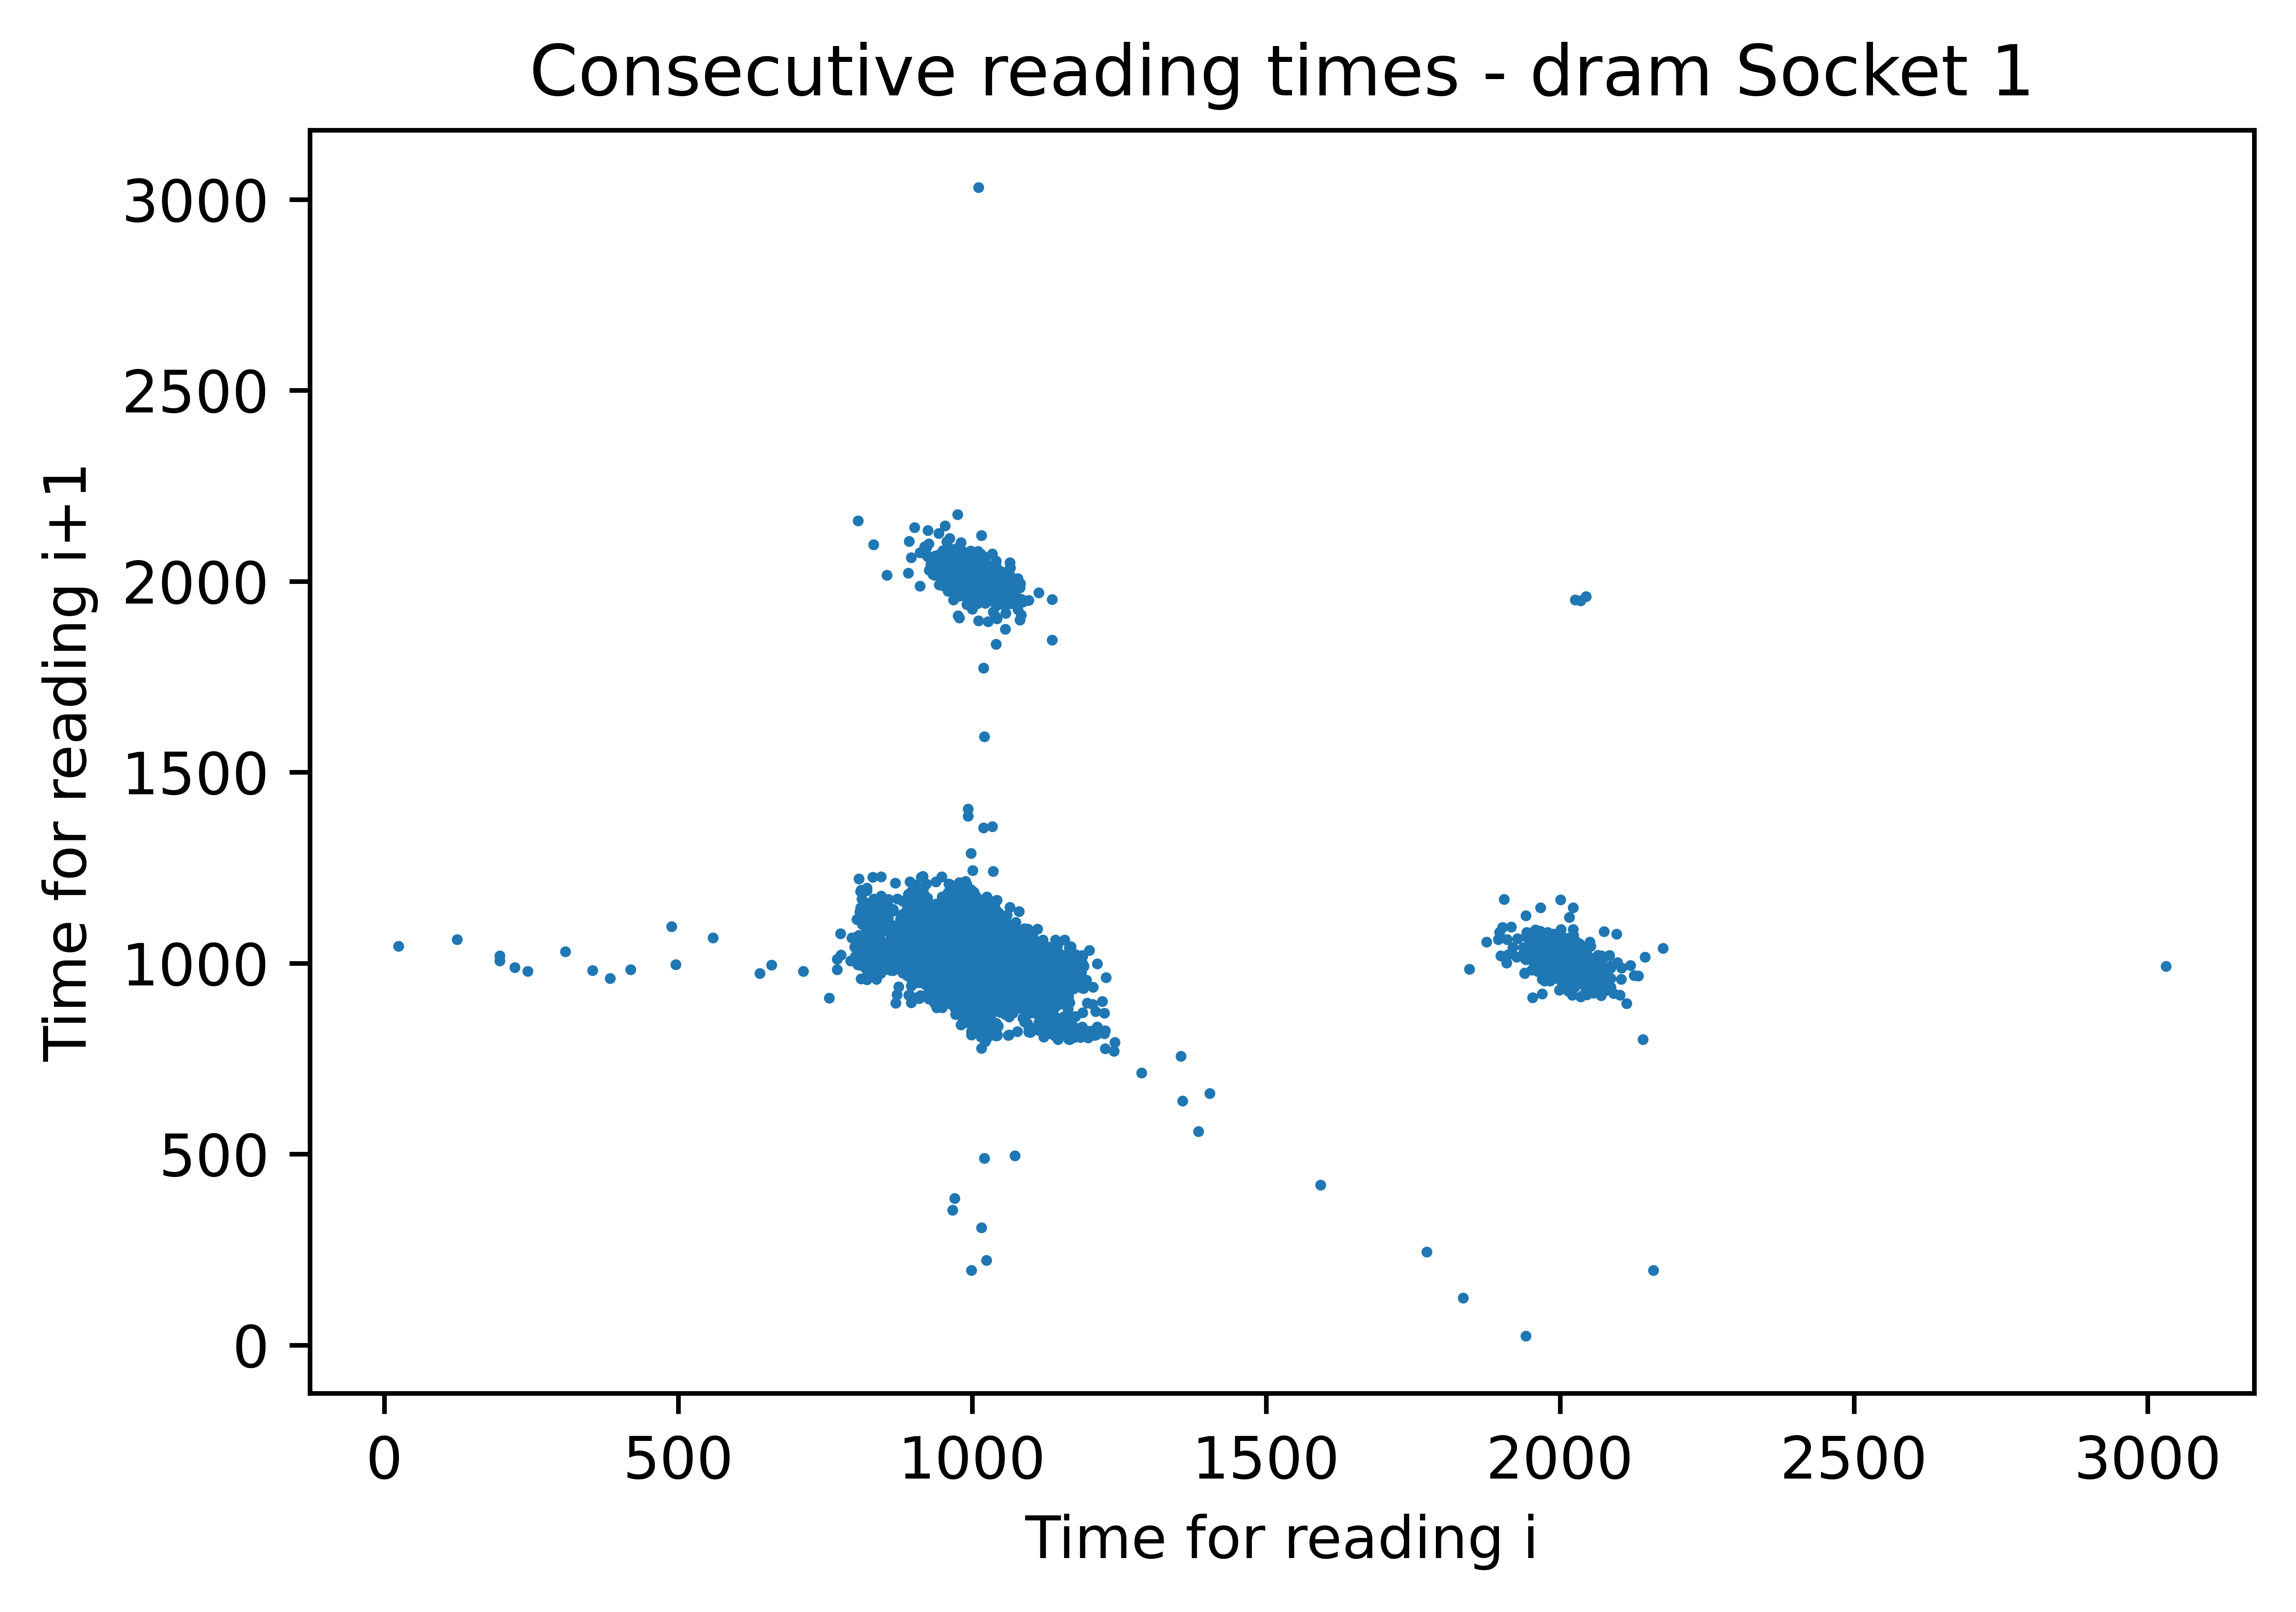
\includegraphics[width=10cm,height=10cm,keepaspectratio]{jmh/msr-update-rate/dram_Socket_1-i_n-v-i_n1.png}
    \caption{How long it takes for the PKG\_socket2 MSR to update (microseconds)}
    \label{fig:PKG-rapl-counter}
\end{figure}

\begin{figure}[H]
    \centering
    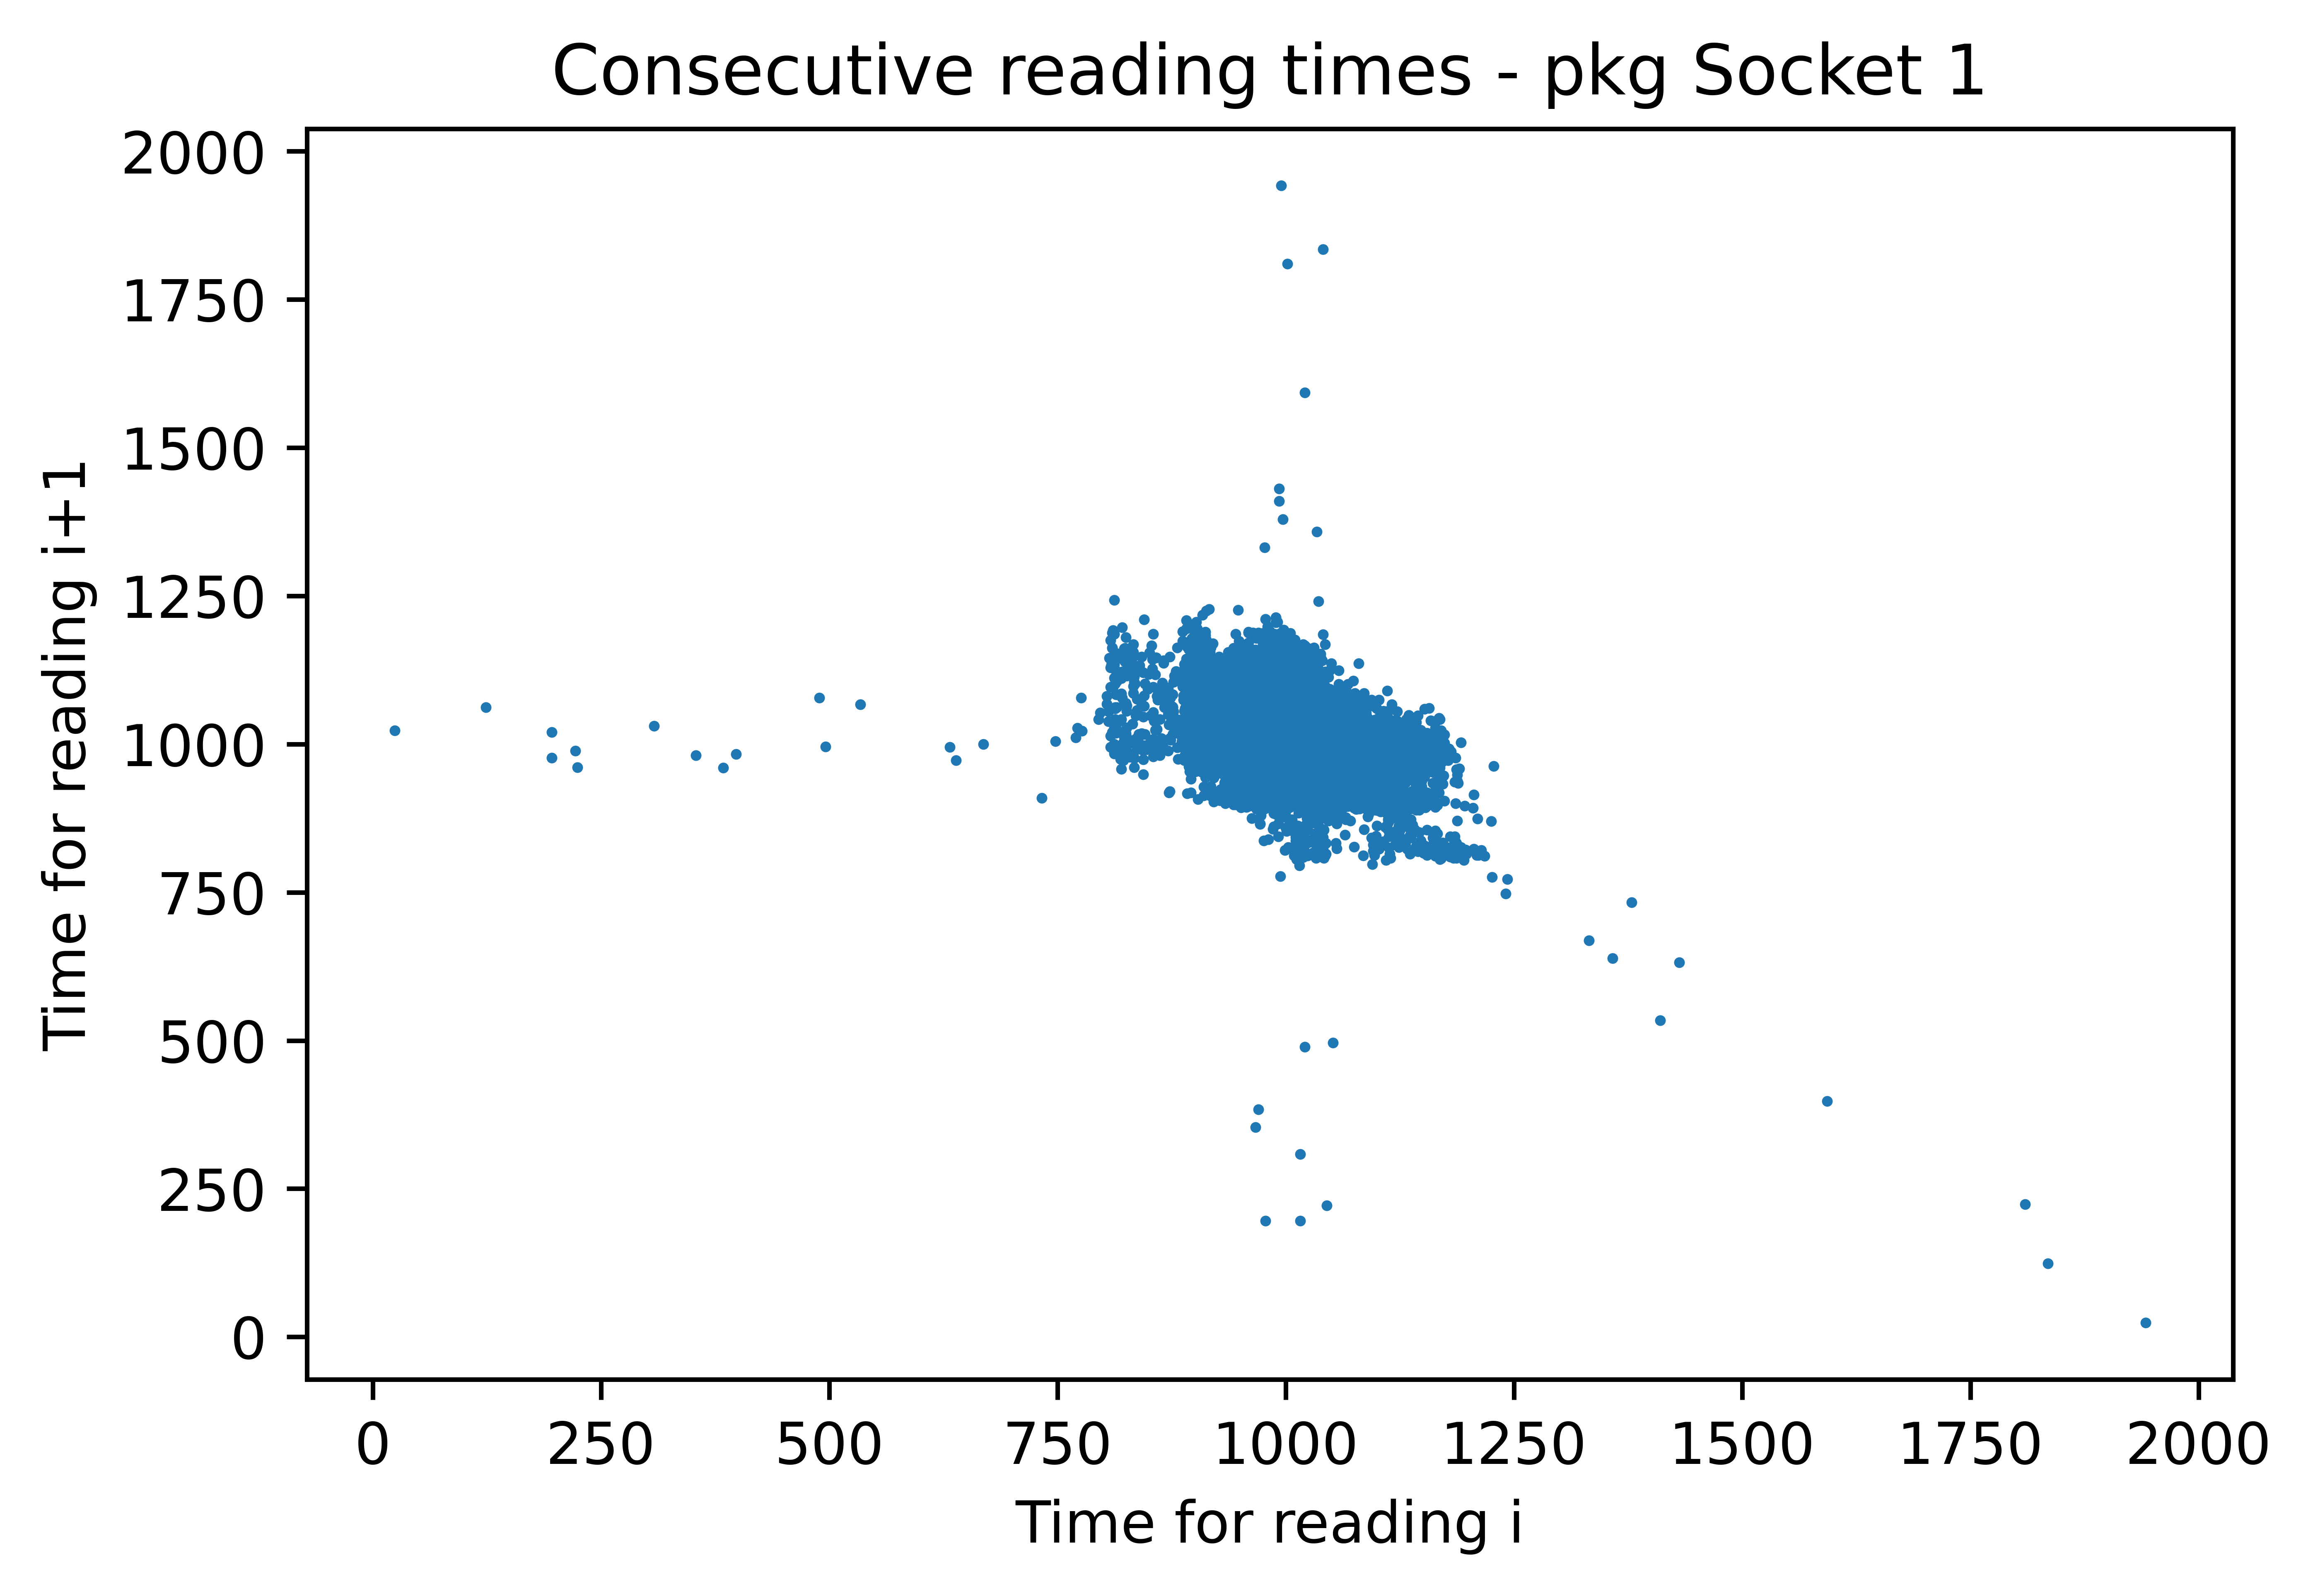
\includegraphics[width=10cm,height=10cm,keepaspectratio]{jmh/msr-update-rate/pkg_Socket_1-i_n-v-i_n1.png}
    \caption{How long it takes for the PKG\_socket2 MSR to update (microseconds)}
    \label{fig:PKG-rapl-counter}
\end{figure}

\begin{figure}[H]
    \centering
    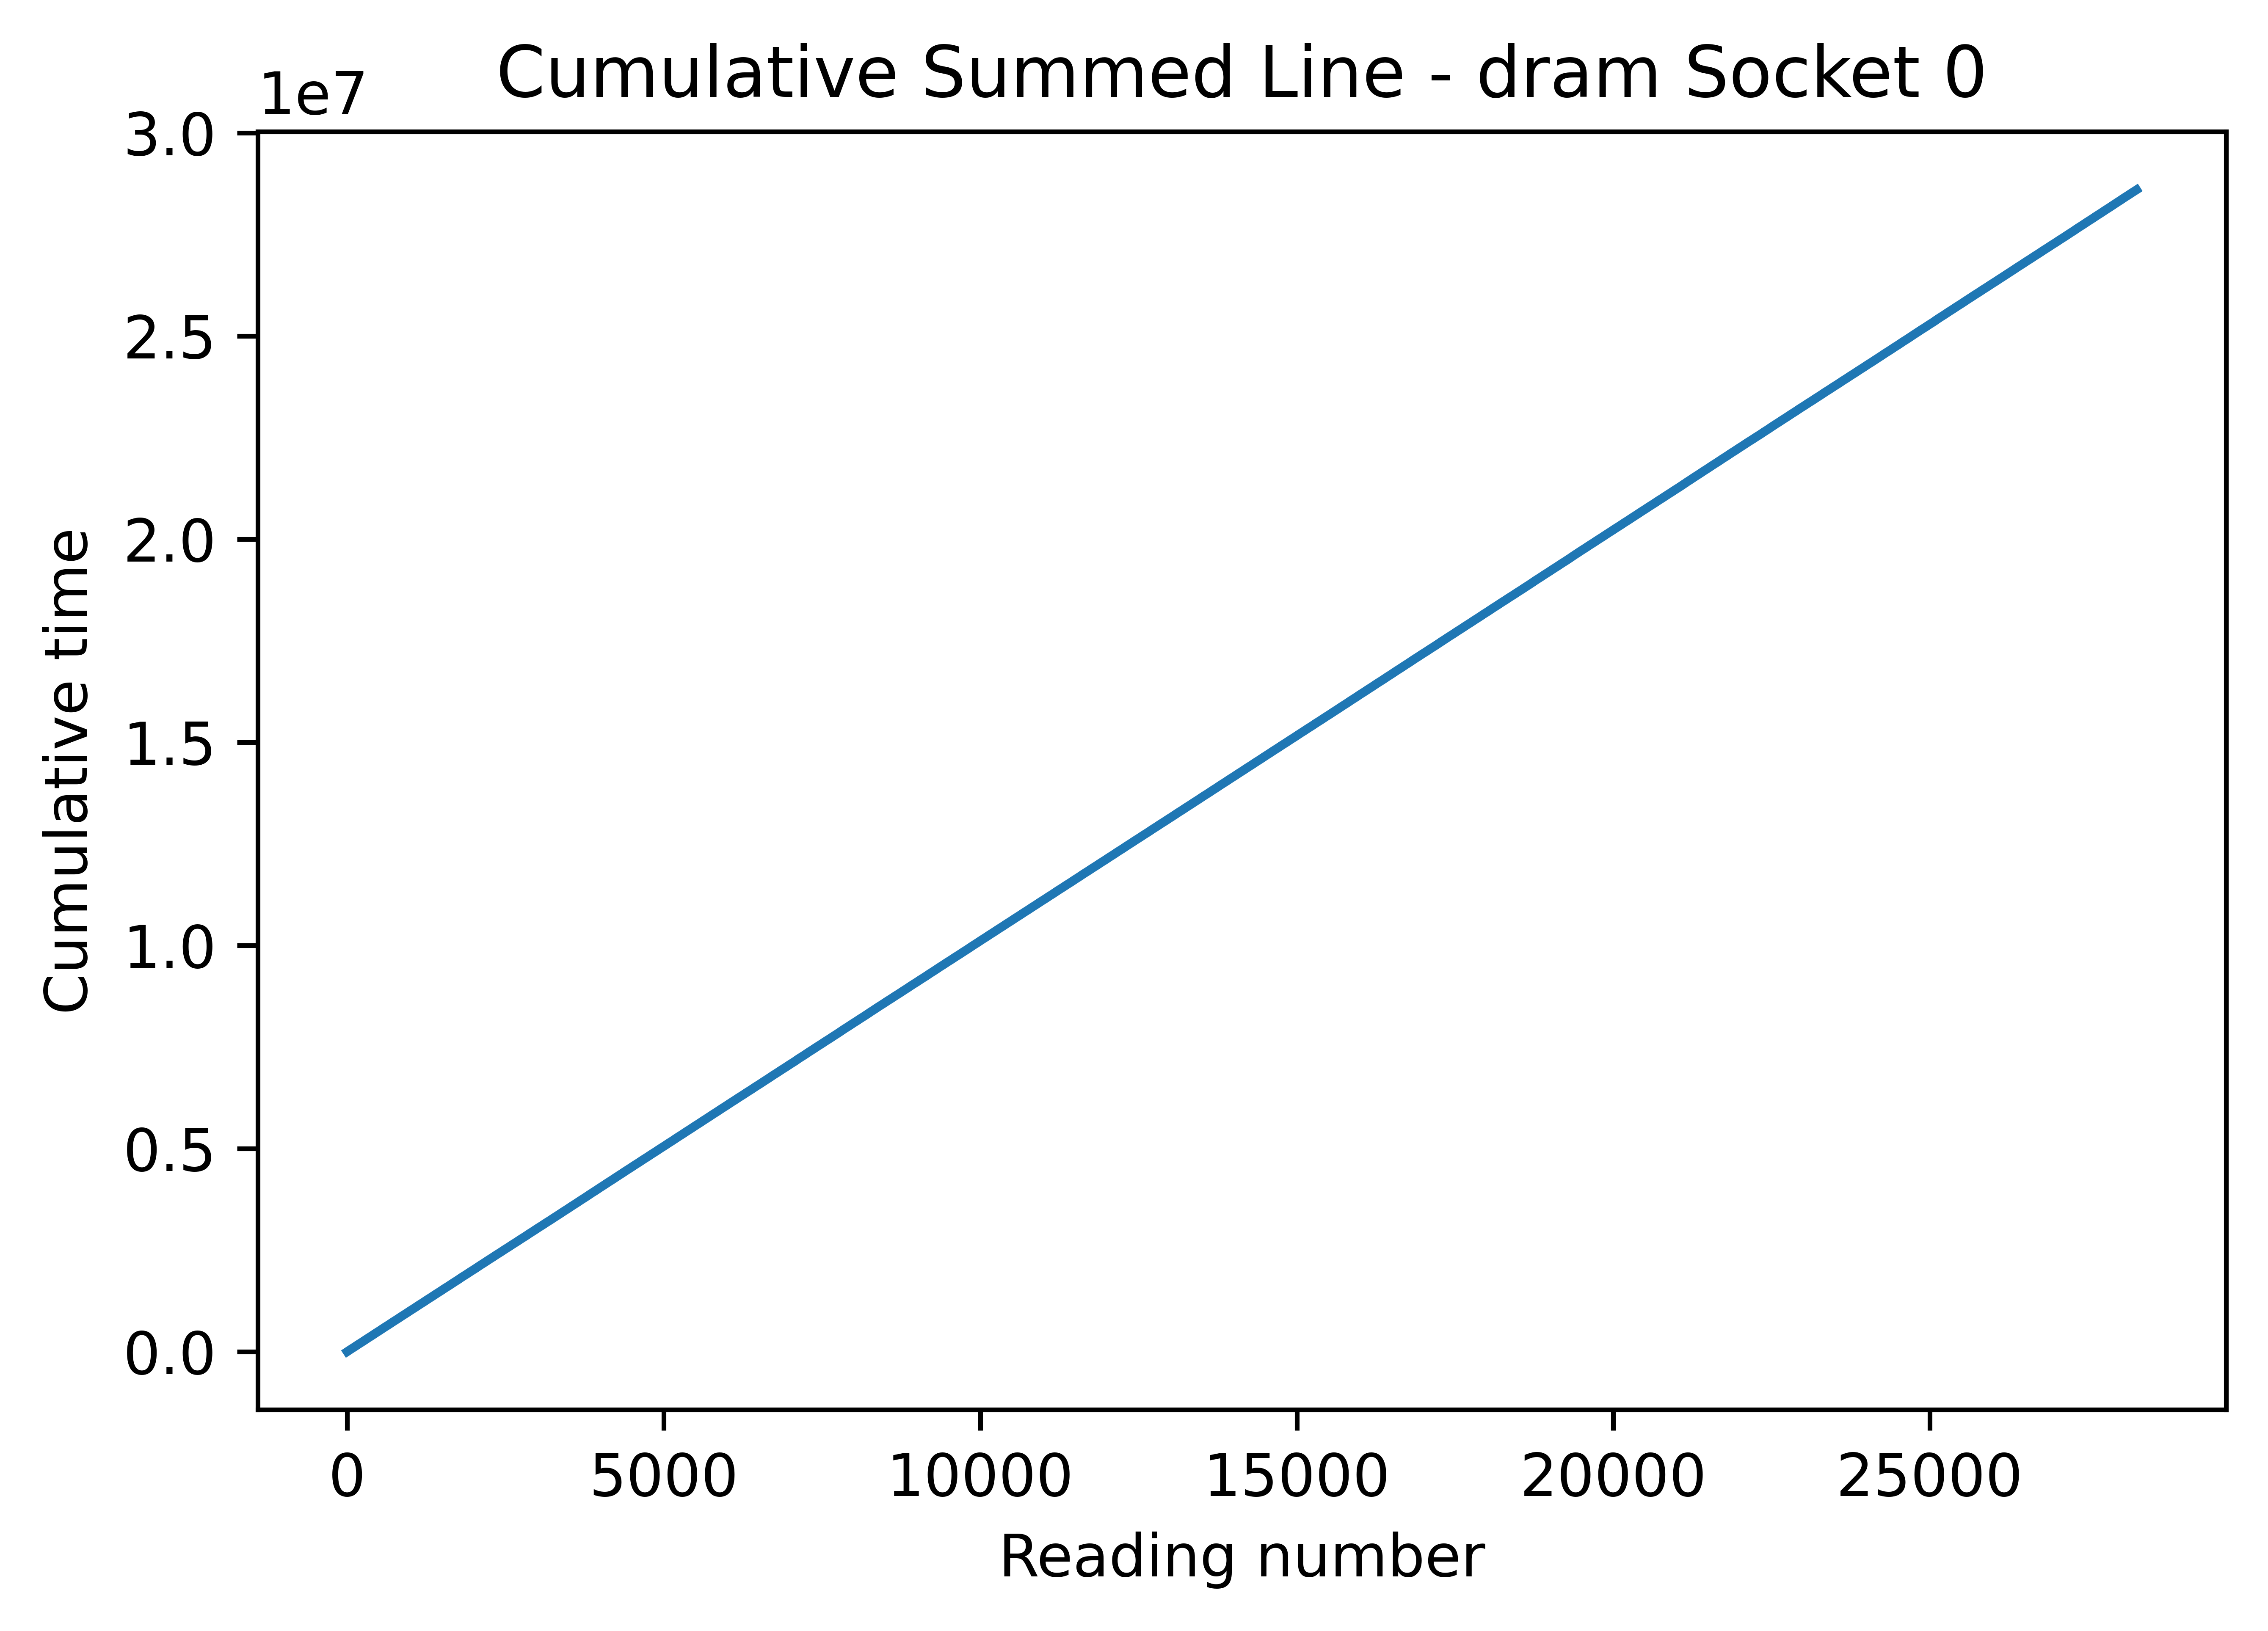
\includegraphics[width=10cm,height=10cm,keepaspectratio]{jmh/msr-update-rate/dram_Socket_0-cumulative-summed.png}
    \caption{How long it takes for the PKG\_socket2 MSR to update (microseconds)}
    \label{fig:PKG-rapl-counter}
\end{figure}

\begin{figure}[H]
    \centering
    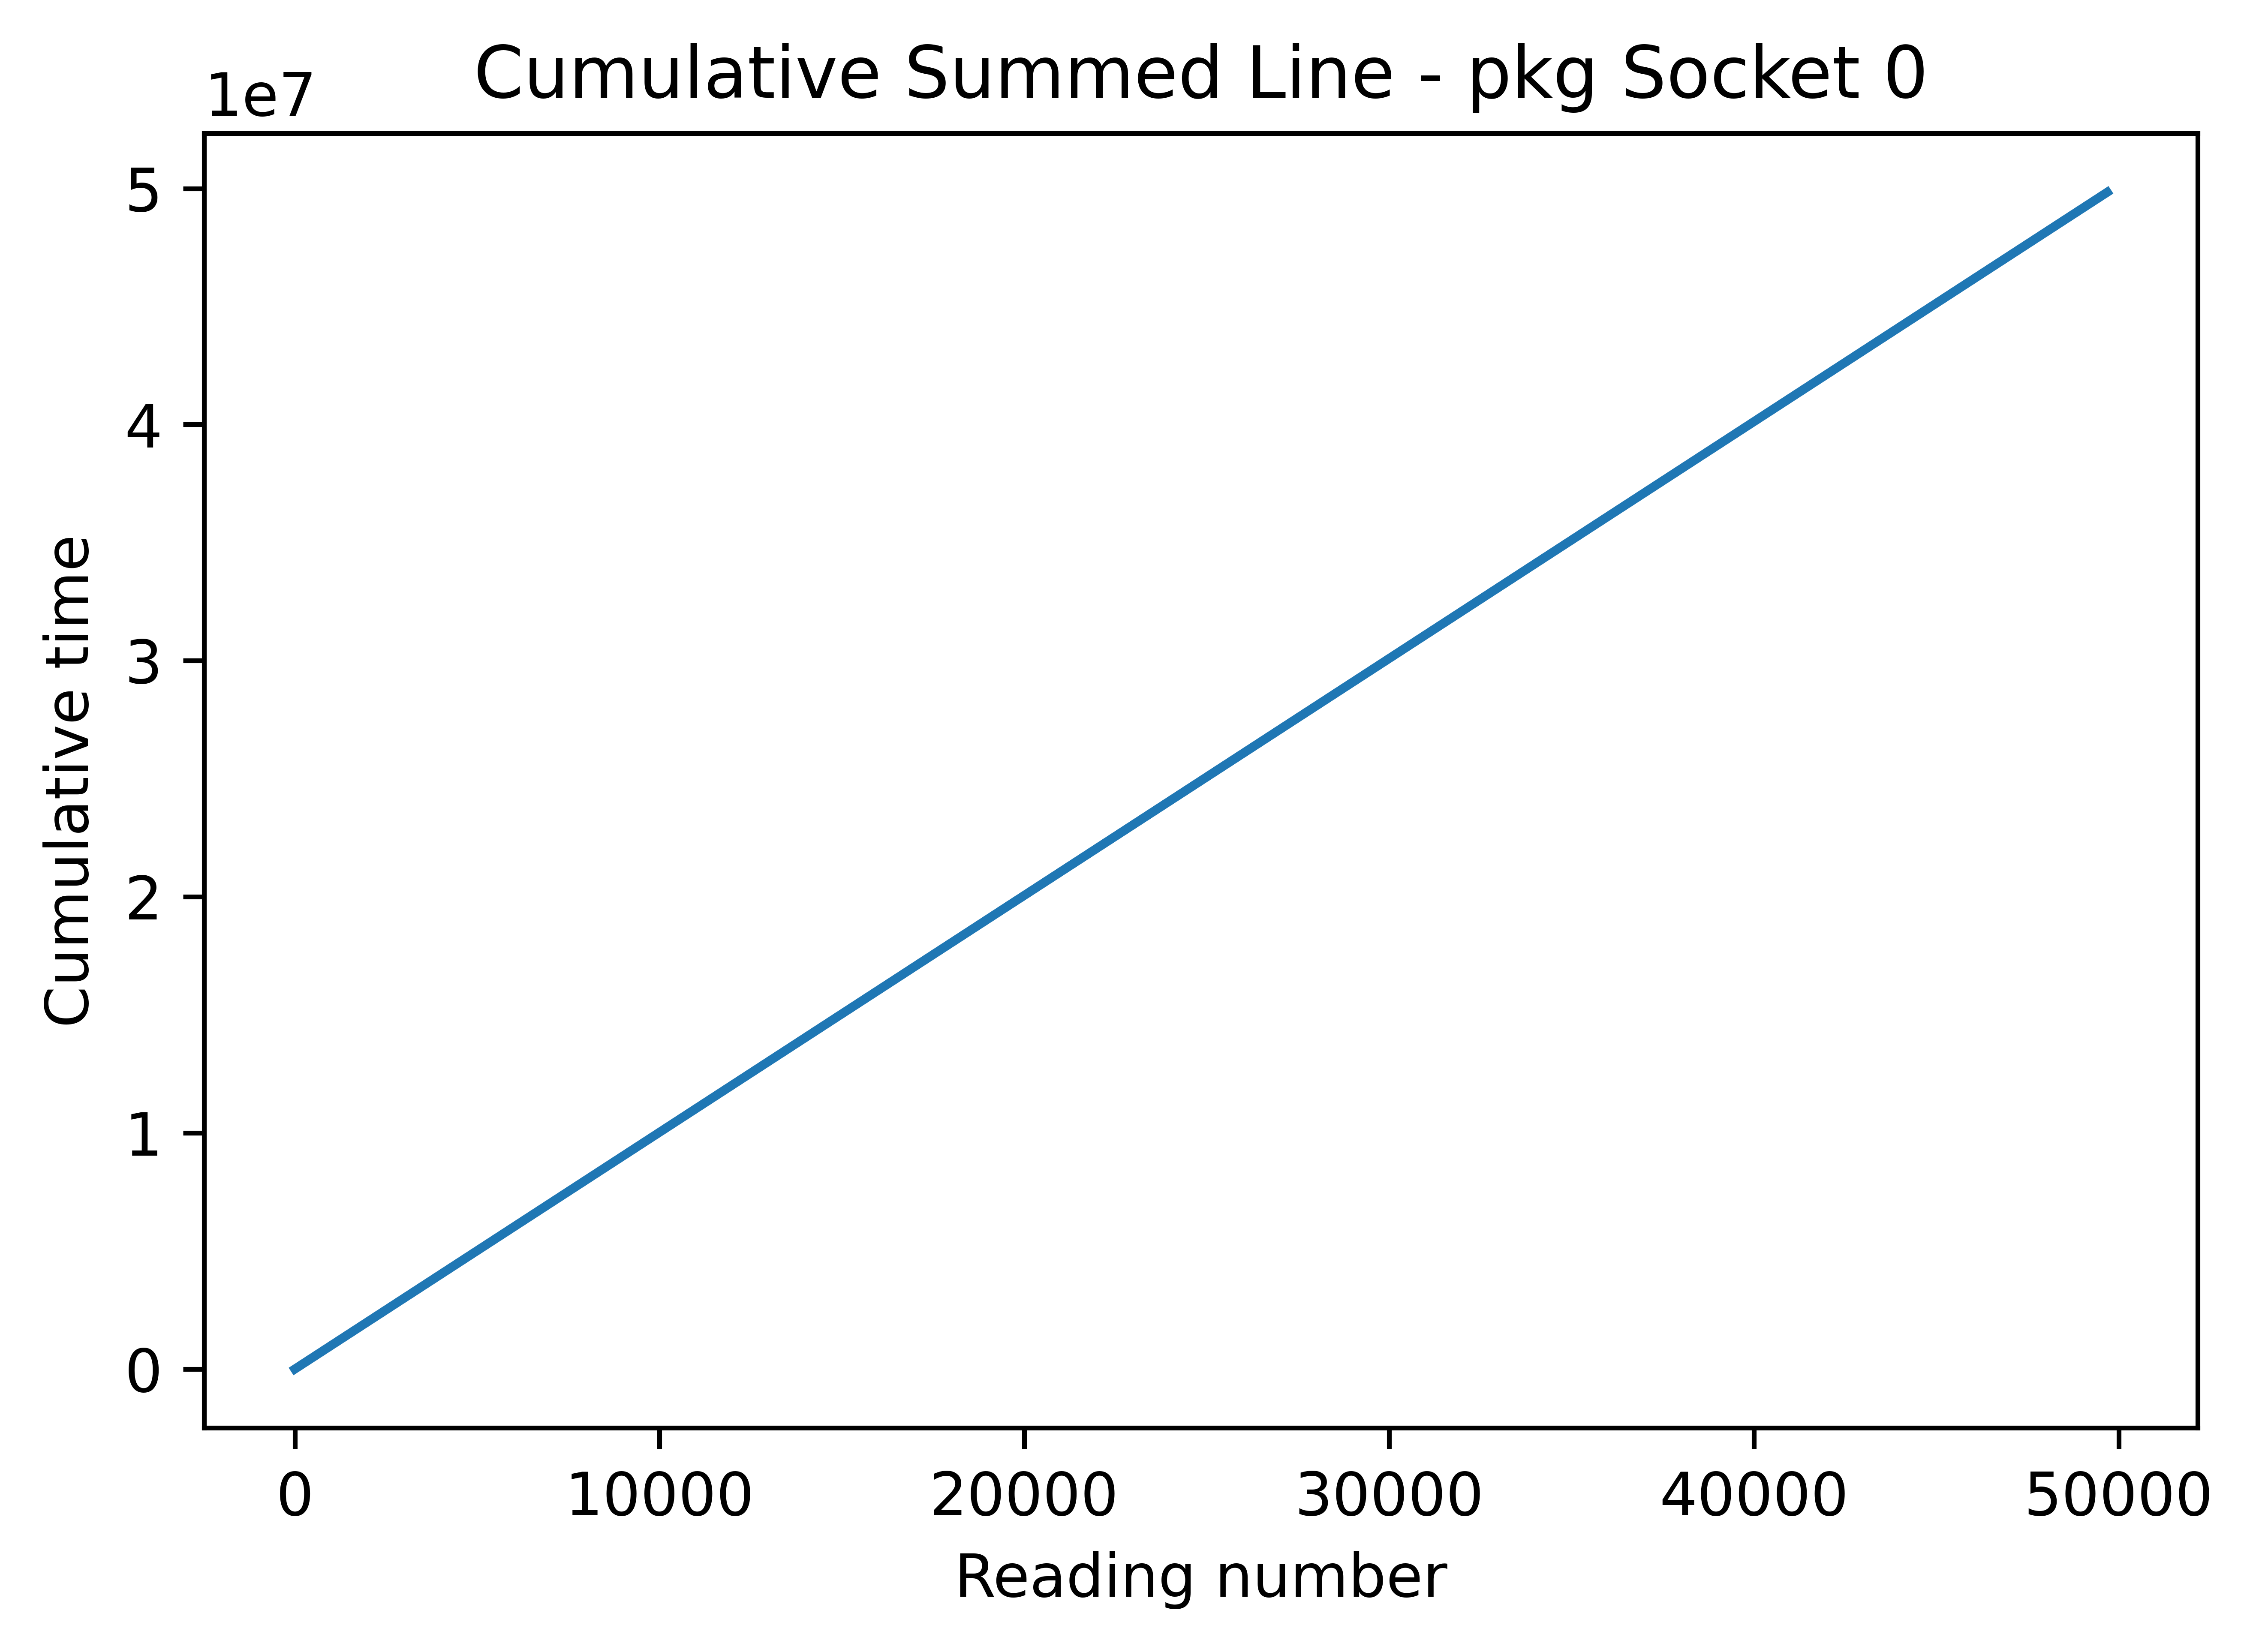
\includegraphics[width=10cm,height=10cm,keepaspectratio]{jmh/msr-update-rate/pkg_Socket_0-cumulative-summed.png}
    \caption{How long it takes for the PKG\_socket2 MSR to update (microseconds)}
    \label{fig:PKG-rapl-counter}
\end{figure}

\begin{figure}[H]
    \centering
    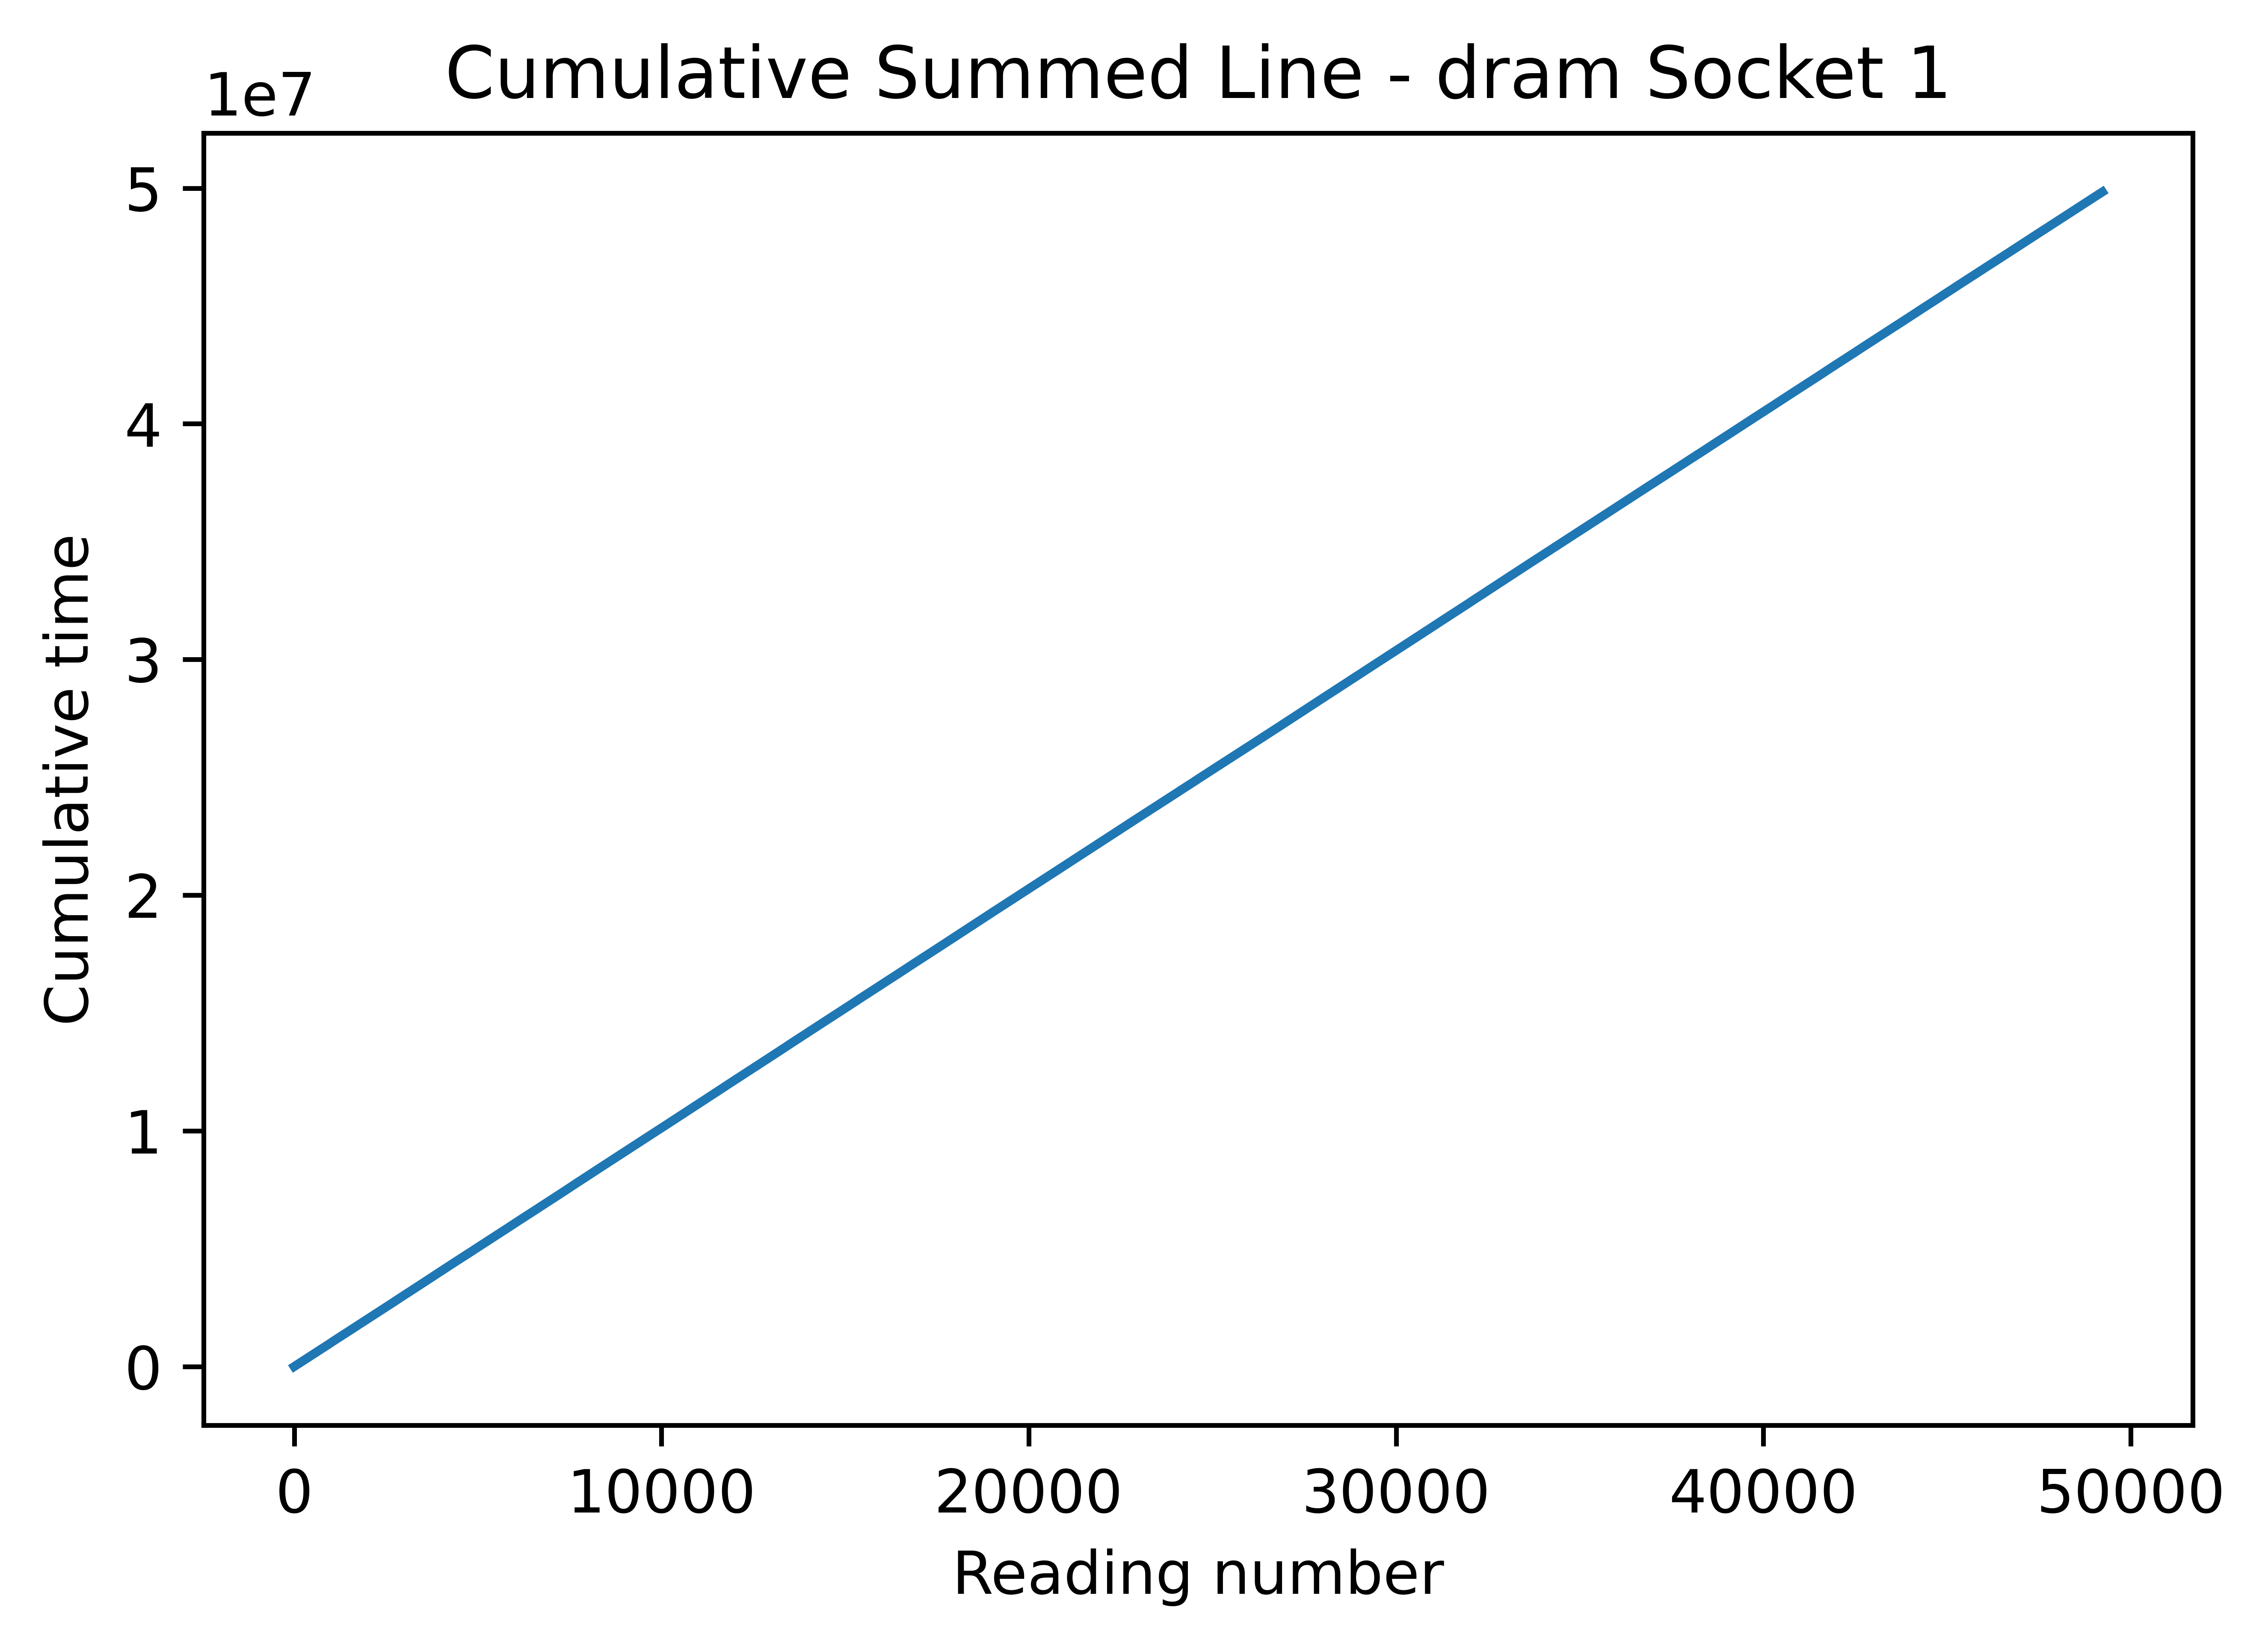
\includegraphics[width=10cm,height=10cm,keepaspectratio]{jmh/msr-update-rate/dram_Socket_1-cumulative-summed.png}
    \caption{How long it takes for the PKG\_socket2 MSR to update (microseconds)}
    \label{fig:PKG-rapl-counter}
\end{figure}

\begin{figure}[H]
    \centering
    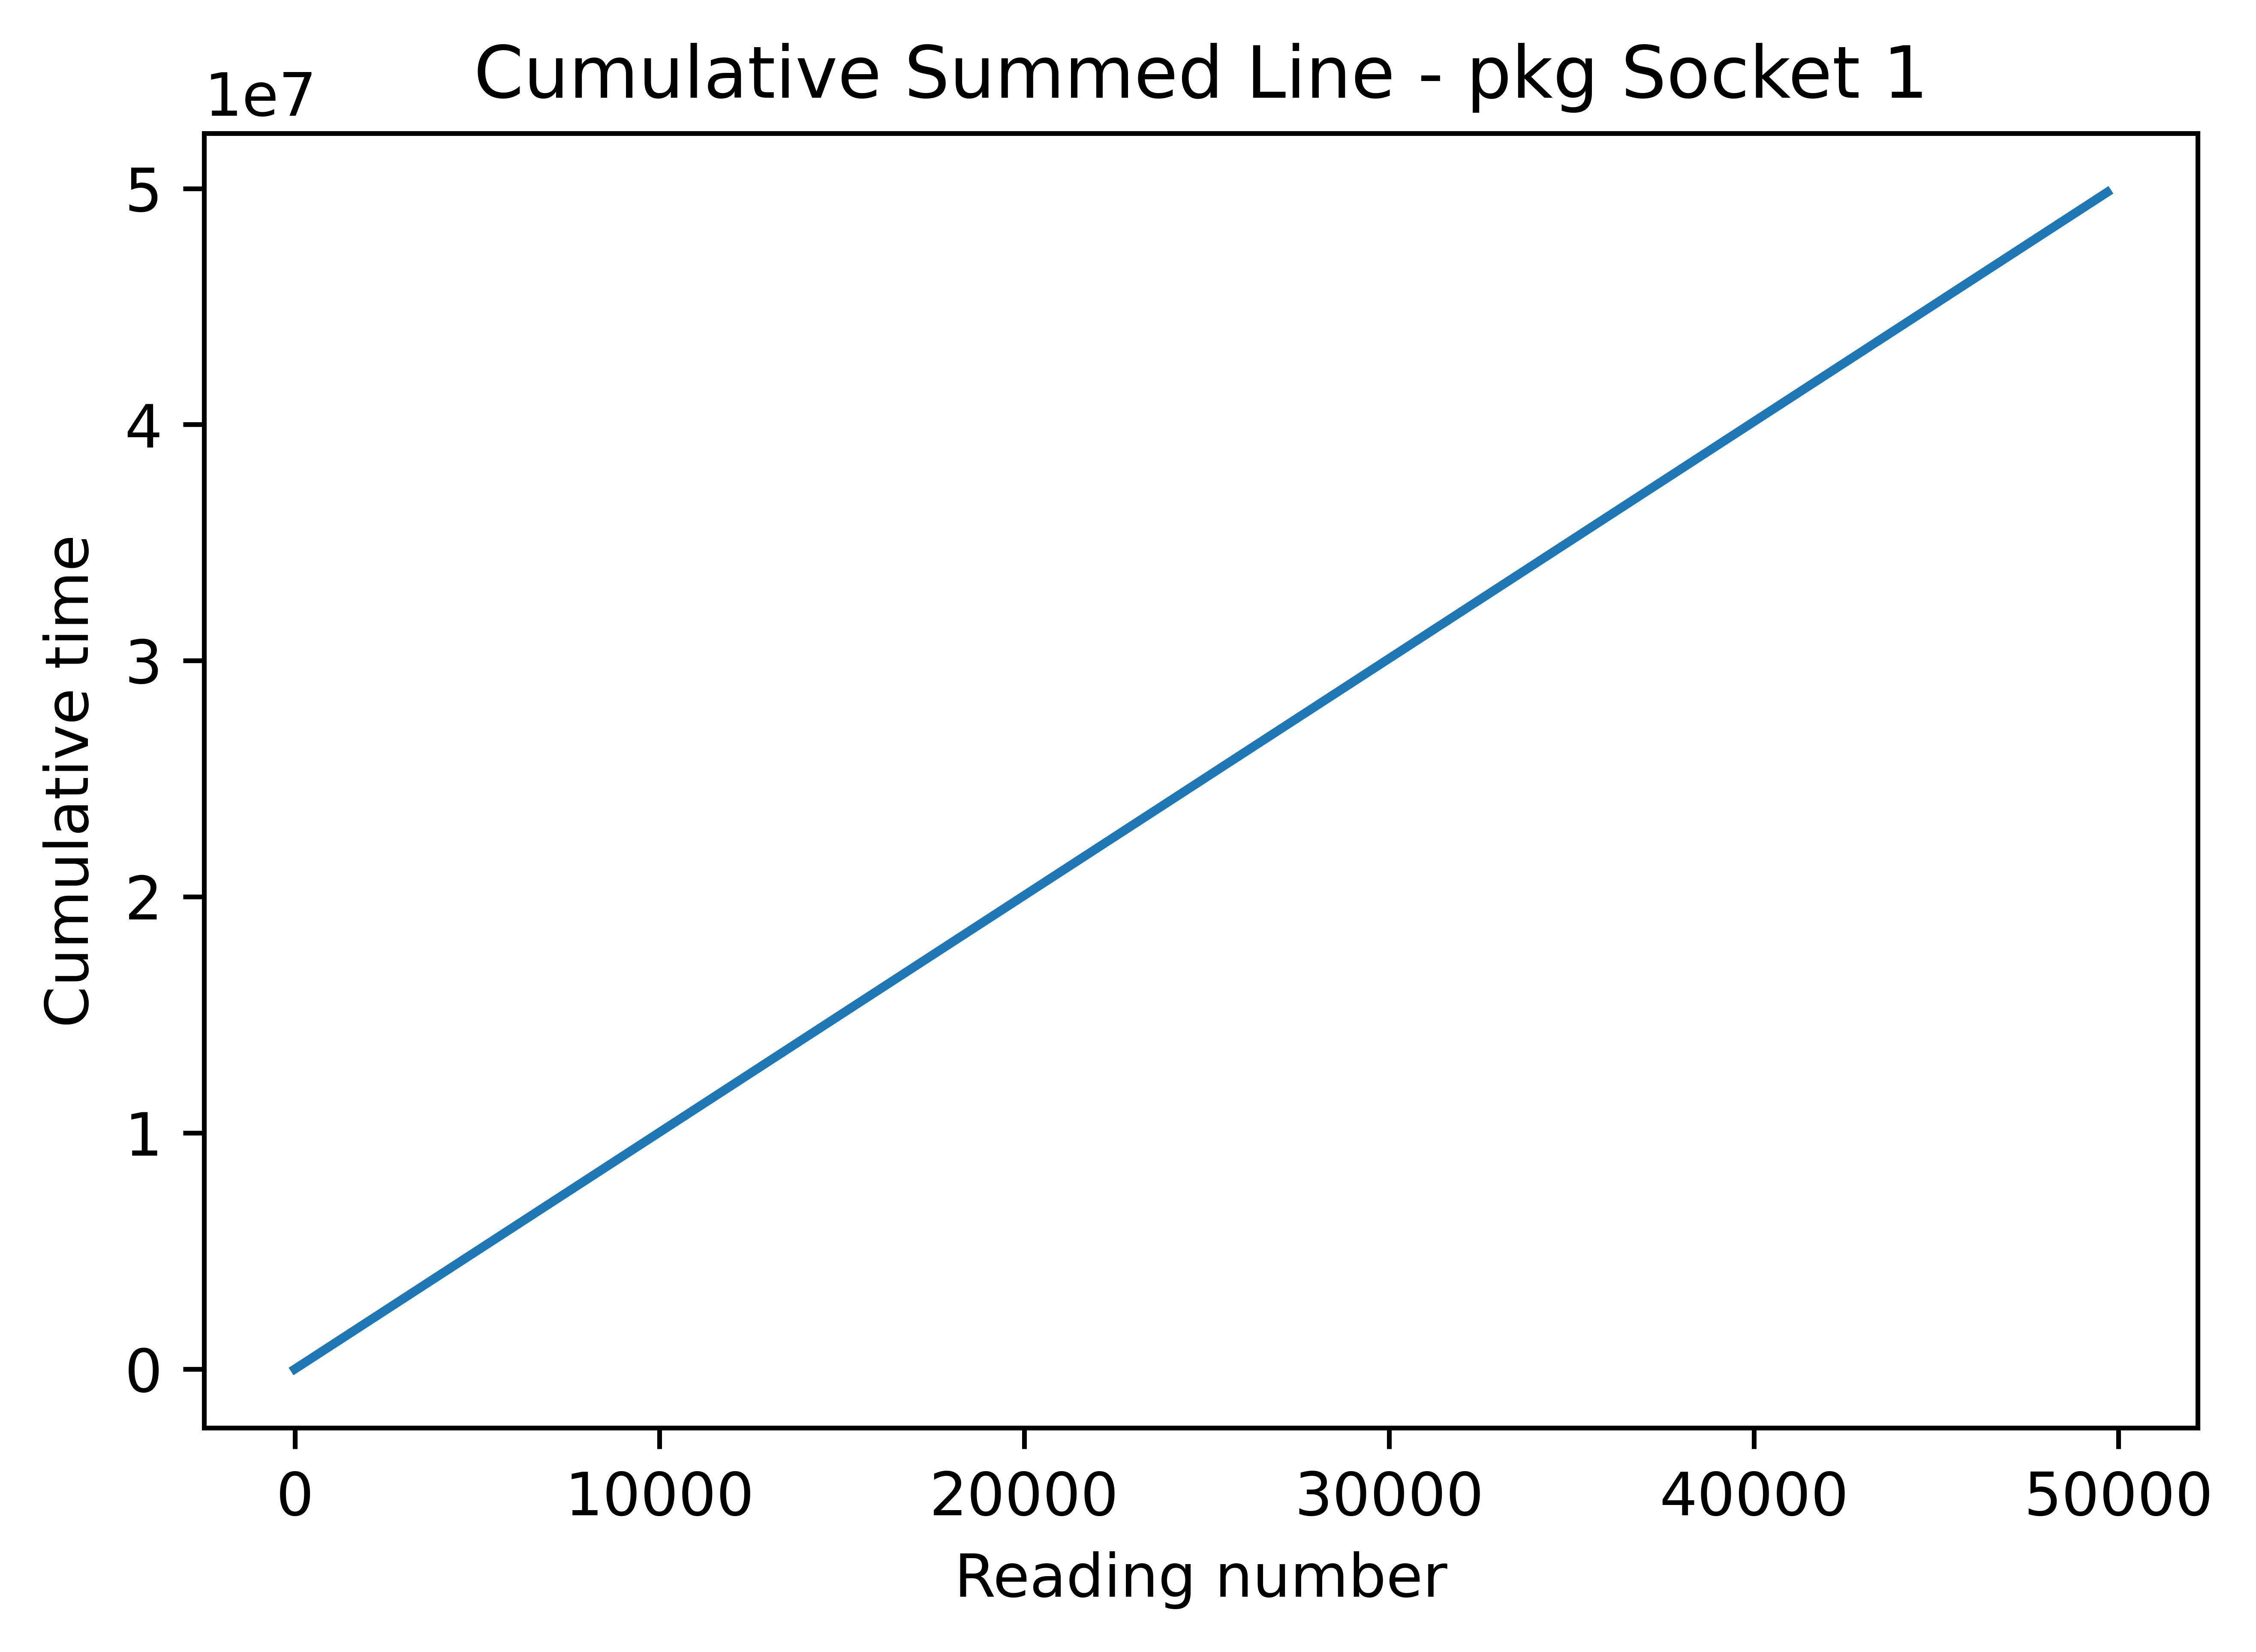
\includegraphics[width=10cm,height=10cm,keepaspectratio]{jmh/msr-update-rate/pkg_Socket_1-cumulative-summed.png}
    \caption{How long it takes for the PKG\_socket2 MSR to update (microseconds)}
    \label{fig:PKG-rapl-counter}
\end{figure}

Dram Socket 0
%\begin{tabular}{lr}
\toprule
{} &   dram_Socket_0_stats \\
ener_diff-vs-num_samples_bw_nonequal & 0.09196352210370197 \\
unique_reading_num-vs-num_samples_bw_nonequal & 0.043276824463455 \\
unique_reading_num-vs-ener_diff & 0.003172218193282899 \\
num_readings & 28367 \\
avg_readings_bw_2_nonequal & 81.62430374391877 \\
s-d_readings_bw_2_nonequal & 884.6362835246799 \\
avg_energy_reading & 0.003991888175985325 \\
s-d_energy_reading & 0.0953152701302277 \\
\bottomrule
\end{tabular}
Dram socket 1
%\begin{tabular}{lr}
\toprule
{} &   dram_Socket_1_stats \\
CC-Energy-Diff-Samples-Between-Non-Equal & -0.020623387258556596 \\
unique_reading_num-vs-num_samples_bw_nonequal & 0.21491816248921825 \\
unique_reading_num-vs-ener_diff & 0.003996556579638411 \\
num_readings & 49240 \\
avg_readings_bw_2_nonequal & 47.180974430837345 \\
s-d_readings_bw_2_nonequal & 6.56195152990962 \\
avg_energy_reading & 0.004011125327484356 \\
s-d_energy_reading & 0.1027373294019606 \\
\bottomrule
\end{tabular}
Pkg Socket 0
%\begin{tabular}{lr}
\toprule
{} &   pkg_Socket_0_stats \\
ener_diff-vs-num_samples_bw_nonequal & -0.06335433066734152 \\
unique_reading_num-vs-num_samples_bw_nonequal & 0.31326217470897305 \\
unique_reading_num-vs-ener_diff & -0.003051859116440657 \\
num_readings & 49699 \\
avg_readings_bw_2_nonequal & 46.73574389311441 \\
s-d_readings_bw_2_nonequal & 4.58756655790207 \\
avg_energy_reading & 0.021698225280695347 \\
s-d_energy_reading & 0.44581372176337347 \\
\bottomrule
\end{tabular}
Pkg Socket 1
%\input{jmh/msr-update-rate/pkg-Socket-1-stats}

\end{document}